%%Section introduction
\intraj\ is our implementation of a precise intraprocedural \CFG\ for Java 7, extending the \intracfg\ framework and the \extendj\ Java compiler.
\intraj\ exploits the \extendj\ front-end, which performs name-, type-, and compile-time error analysis.
\extendj\ produces an attributed AST\footnote{The full abstract grammar for Java 7 can be found at \url{https://extendj.org}} on top of which \intraj\ superimposes the CFG.

In this Section, we discuss the most important design
decisions for \intraj, and in particular, how we used HOAs to improve the precision of the CFG.
%%GOALs
Our two main goals were:
\begin{enumerate}
%%MINIMALITY
\item minimality: build a concise CFG by excluding AST nodes that do not correspond to any runtime action.
This improves client analysis performance, in particular for fixpoint computations.
%%HIGH-PRECISION
\item high precision: the constructed CFGs should capture most program details.
We exploit HOAs to reify implicit structures in the program, such as
calls to static and instance initialisers and implicit conditions in \code{for} loops.
\end{enumerate}
We gave particular importance to exceptions, modelling them as accurately as
possible and weighing the trade-off between precision and minimality.

{\intraj} consists of a total of 989 LOC (598 for Java~4; 11 for Java~5; 380 for Java~7).
We have constructed a systematic benchmark test suite for {\intraj}, consisting of 151 tests in total
(126 for Java~4; 5 for Java 5; 20 for Java~7).
The test suite reads source code as input and produces {\CFG}s as \texttt{dot} files as output.
We validated the result of each test manually.

\subsection{Statements and Expressions}
\label{sec:stmtexp}
When a language implementer specialises \intracfg{} for a given language,
they must decide which AST nodes should be part of the \CFG, i.e., mix in (implement) the \astnode{CFGNode} interface.
As a general design principle, we included AST nodes that correspond to a single action at runtime.
This includes operations on values, like additions, comparisons,
%\astnode{PlusExpr} and \astnode{LEExpr}
and read operations on variables and fields.
%, e.g, \astnode{VarAccess}.

We also included nodes that are interesting points in the execution that a client analysis might want to use.
This includes nodes that redirect flow outside of the CFG, like method calls, return statements, and throw statements.
%\astnode{MethodAccess}, \astnode{ReturnStmt}, and \astnode{ThrowStmt}.

For assignments, the choice of nodes to include in the \CFG\ was not obvious.
The left-hand side of an assignment can be a chain of named accesses and method calls, e.g., \code{f.m().x}, with the rightmost named access, \code{x}, corresponding to the write.
% (the l-value of the assignment).
Here, we chose to not include \code{x} in the \CFG\, but instead use the assignment node itself
%(\astnode{AssignExpr})
to represent the write operation, see Figure~\ref{fig:AssigExpr}.
We argue that this gives a simpler client interface, since the same AST node type, \astnode{VarAccess}, otherwise represents all named accesses on the left- and right-hand side of an assignment.
%regardless of if they represent a read or a write operation.
% \todo{I removed mentioning of package. It is not in the example, and should probably not be a CFG node anyway. /GH}

\begin{figure}
   \scalebox{0.60}{
     

\tikzset{every picture/.style={line width=0.75pt}} %set default line width to 0.75pt
\tikzset{
pattern size/.store in=\mcSize,
pattern size = 5pt,
pattern thickness/.store in=\mcThickness,
pattern thickness = 0.3pt,
pattern radius/.store in=\mcRadius,
pattern radius = 1pt}
\makeatletter
\pgfutil@ifundefined{pgf@pattern@name@_27w6fw9du}{
\pgfdeclarepatternformonly[\mcThickness,\mcSize]{_27w6fw9du}
{\pgfqpoint{0pt}{-\mcThickness}}
{\pgfpoint{\mcSize}{\mcSize}}
{\pgfpoint{\mcSize}{\mcSize}}
{
\pgfsetcolor{\tikz@pattern@color}
\pgfsetlinewidth{\mcThickness}
\pgfpathmoveto{\pgfqpoint{0pt}{\mcSize}}
\pgfpathlineto{\pgfpoint{\mcSize+\mcThickness}{-\mcThickness}}
\pgfusepath{stroke}
}}
\makeatother
\begin{tikzpicture}[x=0.75pt,y=0.75pt,yscale=-1,xscale=1]
%uncomment if require: \path (0,705); %set diagram left start at 0, and has height of 705

%Rounded Rect [id:dp7903090714997506]
\draw  [fill={rgb, 255:red, 255; green, 255; blue, 255 }  ,fill opacity=1 ] (95.5,127.04) .. controls (95.5,124.32) and (97.7,122.12) .. (100.41,122.12) -- (195.18,122.12) .. controls (197.9,122.12) and (200.1,124.32) .. (200.1,127.04) -- (200.1,141.79) .. controls (200.1,144.5) and (197.9,146.7) .. (195.18,146.7) -- (100.41,146.7) .. controls (97.7,146.7) and (95.5,144.5) .. (95.5,141.79) -- cycle ;
%Straight Lines [id:da9706544646184255]
\draw  [dash pattern={on 0.84pt off 2.51pt}]  (146.89,147.38) -- (146.89,155.96) -- (134.12,169.79) ;
\draw [shift={(132.76,171.26)}, rotate = 312.72] [fill={rgb, 255:red, 0; green, 0; blue, 0 }  ][line width=0.08]  [draw opacity=0] (12,-3) -- (0,0) -- (12,3) -- cycle    ;
%Straight Lines [id:da9042513300440475]
\draw  [dash pattern={on 0.84pt off 2.51pt}]  (146.89,147.38) -- (146.67,155.33) -- (157.13,169.65) ;
\draw [shift={(158.31,171.26)}, rotate = 233.82] [fill={rgb, 255:red, 0; green, 0; blue, 0 }  ][line width=0.08]  [draw opacity=0] (12,-3) -- (0,0) -- (12,3) -- cycle    ;
%Rounded Rect [id:dp7484538791357932]
\draw  [fill={rgb, 255:red, 224; green, 219; blue, 219 }  ,fill opacity=1 ] (78.73,176.14) .. controls (78.73,173.08) and (81.21,170.61) .. (84.27,170.61) -- (129.42,170.61) .. controls (132.48,170.61) and (134.96,173.08) .. (134.96,176.14) -- (134.96,192.75) .. controls (134.96,195.81) and (132.48,198.29) .. (129.42,198.29) -- (84.27,198.29) .. controls (81.21,198.29) and (78.73,195.81) .. (78.73,192.75) -- cycle ;
%Rounded Rect [id:dp4276430409681904]
\draw  [fill={rgb, 255:red, 224; green, 219; blue, 219 }  ,fill opacity=1 ] (114.67,229.39) .. controls (114.67,226.33) and (117.15,223.86) .. (120.21,223.86) -- (165.36,223.86) .. controls (168.42,223.86) and (170.9,226.33) .. (170.9,229.39) -- (170.9,246) .. controls (170.9,249.06) and (168.42,251.54) .. (165.36,251.54) -- (120.21,251.54) .. controls (117.15,251.54) and (114.67,249.06) .. (114.67,246) -- cycle ;
%Rounded Rect [id:dp6223290375474622]
\draw   (1.5,230.18) .. controls (1.5,225.72) and (5.12,222.1) .. (9.59,222.1) -- (81.41,222.1) .. controls (85.88,222.1) and (89.5,225.72) .. (89.5,230.18) -- (89.5,254.44) .. controls (89.5,258.91) and (85.88,262.53) .. (81.41,262.53) -- (9.59,262.53) .. controls (5.12,262.53) and (1.5,258.91) .. (1.5,254.44) -- cycle ;
%Rounded Rect [id:dp10276274539512309]
\draw   (10.94,290.77) .. controls (10.94,286.75) and (14.19,283.5) .. (18.21,283.5) -- (117.43,283.5) .. controls (121.45,283.5) and (124.7,286.75) .. (124.7,290.77) -- (124.7,312.56) .. controls (124.7,316.58) and (121.45,319.83) .. (117.43,319.83) -- (18.21,319.83) .. controls (14.19,319.83) and (10.94,316.58) .. (10.94,312.56) -- cycle ;
%Straight Lines [id:da644954294752564]
\draw  [dash pattern={on 0.84pt off 2.51pt}]  (106.19,198.85) -- (106.23,208.53) -- (84.92,220.37) ;
\draw [shift={(83.17,221.34)}, rotate = 330.96000000000004] [fill={rgb, 255:red, 0; green, 0; blue, 0 }  ][line width=0.08]  [draw opacity=0] (12,-3) -- (0,0) -- (12,3) -- cycle    ;
%Straight Lines [id:da3821451488528739]
\draw  [dash pattern={on 0.84pt off 2.51pt}]  (106.19,198.85) -- (106.23,208.53) -- (123.6,218.47) ;
\draw [shift={(125.34,219.46)}, rotate = 209.77] [fill={rgb, 255:red, 0; green, 0; blue, 0 }  ][line width=0.08]  [draw opacity=0] (12,-3) -- (0,0) -- (12,3) -- cycle    ;
%Straight Lines [id:da2083023707056817]
\draw  [dash pattern={on 0.84pt off 2.51pt}]  (143.62,253.74) -- (143.66,261.66) -- (118.97,282.22) ;
\draw [shift={(117.43,283.5)}, rotate = 320.22] [fill={rgb, 255:red, 0; green, 0; blue, 0 }  ][line width=0.08]  [draw opacity=0] (12,-3) -- (0,0) -- (12,3) -- cycle    ;
%Straight Lines [id:da9703636123816585]
\draw  [dash pattern={on 0.84pt off 2.51pt}]  (143.62,253.74) -- (143.66,261.66) -- (165.23,274.67) ;
\draw [shift={(166.94,275.7)}, rotate = 211.11] [fill={rgb, 255:red, 0; green, 0; blue, 0 }  ][line width=0.08]  [draw opacity=0] (12,-3) -- (0,0) -- (12,3) -- cycle    ;
%Rounded Rect [id:dp8370202719972792]
\draw  [fill={rgb, 255:red, 255; green, 255; blue, 255 }  ,fill opacity=1 ] (157.5,178.74) .. controls (157.5,174.55) and (160.89,171.16) .. (165.08,171.16) -- (255.92,171.16) .. controls (260.11,171.16) and (263.5,174.55) .. (263.5,178.74) -- (263.5,201.48) .. controls (263.5,205.66) and (260.11,209.05) .. (255.92,209.05) -- (165.08,209.05) .. controls (160.89,209.05) and (157.5,205.66) .. (157.5,201.48) -- cycle ;
%Straight Lines [id:da12282371980602014]
\draw [color={rgb, 255:red, 74; green, 144; blue, 226 }  ,draw opacity=1 ][line width=1.5]    (48.99,263.7) -- (48.99,279.22) ;
\draw [shift={(48.99,283.22)}, rotate = 270] [fill={rgb, 255:red, 74; green, 144; blue, 226 }  ,fill opacity=1 ][line width=0.08]  [draw opacity=0] (11.61,-5.58) -- (0,0) -- (11.61,5.58) -- cycle    ;
%Straight Lines [id:da8947984177896998]
\draw [color={rgb, 255:red, 74; green, 144; blue, 226 }  ,draw opacity=1 ][line width=1.5]    (127.94,299.29) -- (143.94,299.29) -- (208.94,239.7) -- (208.94,220.7) ;
\draw [shift={(208.94,216.7)}, rotate = 450] [fill={rgb, 255:red, 74; green, 144; blue, 226 }  ,fill opacity=1 ][line width=0.08]  [draw opacity=0] (11.61,-5.58) -- (0,0) -- (11.61,5.58) -- cycle    ;
%Straight Lines [id:da32622503119057666]
\draw [color={rgb, 255:red, 74; green, 144; blue, 226 }  ,draw opacity=1 ][line width=1.5]    (247.67,170.33) -- (247.17,141.46) -- (206.81,141.46) ;
\draw [shift={(202.81,141.46)}, rotate = 360] [fill={rgb, 255:red, 74; green, 144; blue, 226 }  ,fill opacity=1 ][line width=0.08]  [draw opacity=0] (11.61,-5.58) -- (0,0) -- (11.61,5.58) -- cycle    ;
%Rounded Rect [id:dp6982924691250458]
\draw  [fill={rgb, 255:red, 119; green, 119; blue, 119 }  ,fill opacity=1 ] (107.5,14.8) .. controls (107.5,11.6) and (110.1,9) .. (113.3,9) -- (184.7,9) .. controls (187.9,9) and (190.5,11.6) .. (190.5,14.8) -- (190.5,32.2) .. controls (190.5,35.4) and (187.9,38) .. (184.7,38) -- (113.3,38) .. controls (110.1,38) and (107.5,35.4) .. (107.5,32.2) -- cycle ;
%Rounded Rect [id:dp9930154822954091]
\draw  [dash pattern={on 4.5pt off 4.5pt}] (44.5,58.21) .. controls (44.5,55.15) and (46.98,52.68) .. (50.04,52.68) -- (95.19,52.68) .. controls (98.25,52.68) and (100.73,55.15) .. (100.73,58.21) -- (100.73,74.82) .. controls (100.73,77.88) and (98.25,80.36) .. (95.19,80.36) -- (50.04,80.36) .. controls (46.98,80.36) and (44.5,77.88) .. (44.5,74.82) -- cycle ;
%Rounded Rect [id:dp3998391789510459]
\draw  [dash pattern={on 4.5pt off 4.5pt}] (201.41,58.33) .. controls (201.41,55.28) and (203.89,52.8) .. (206.94,52.8) -- (252.09,52.8) .. controls (255.15,52.8) and (257.63,55.28) .. (257.63,58.33) -- (257.63,74.95) .. controls (257.63,78) and (255.15,80.48) .. (252.09,80.48) -- (206.94,80.48) .. controls (203.89,80.48) and (201.41,78) .. (201.41,74.95) -- cycle ;
%Straight Lines [id:da7572945714768814]
\draw  [dash pattern={on 0.84pt off 2.51pt}]  (146.97,47.99) -- (104.41,58.09) ;
\draw [shift={(102.47,58.55)}, rotate = 346.64] [fill={rgb, 255:red, 0; green, 0; blue, 0 }  ][line width=0.08]  [draw opacity=0] (12,-3) -- (0,0) -- (12,3) -- cycle    ;
%Straight Lines [id:da15529375781546706]
\draw  [dash pattern={on 0.84pt off 2.51pt}]  (146.93,38.31) -- (146.97,46.99) -- (194.95,57.66) ;
\draw [shift={(196.9,58.09)}, rotate = 192.53] [fill={rgb, 255:red, 0; green, 0; blue, 0 }  ][line width=0.08]  [draw opacity=0] (12,-3) -- (0,0) -- (12,3) -- cycle    ;
%Rounded Rect [id:dp01440000102762784]
\draw  [fill={rgb, 255:red, 224; green, 219; blue, 219 }  ,fill opacity=1 ] (107.59,72.46) .. controls (107.59,69.4) and (110.07,66.92) .. (113.13,66.92) -- (186.05,66.92) .. controls (189.11,66.92) and (191.59,69.4) .. (191.59,72.46) -- (191.59,89.07) .. controls (191.59,92.13) and (189.11,94.61) .. (186.05,94.61) -- (113.13,94.61) .. controls (110.07,94.61) and (107.59,92.13) .. (107.59,89.07) -- cycle ;
%Straight Lines [id:da03365349511935756]
\draw  [dash pattern={on 0.84pt off 2.51pt}]  (146.97,47.99) -- (146.93,61.29) ;
\draw [shift={(146.93,63.29)}, rotate = 270.17] [fill={rgb, 255:red, 0; green, 0; blue, 0 }  ][line width=0.08]  [draw opacity=0] (12,-3) -- (0,0) -- (12,3) -- cycle    ;
%Straight Lines [id:da48895600839842357]
\draw  [dash pattern={on 0.84pt off 2.51pt}]  (148.8,97.93) -- (148.8,116.05) ;
\draw [shift={(148.8,118.05)}, rotate = 270] [fill={rgb, 255:red, 0; green, 0; blue, 0 }  ][line width=0.08]  [draw opacity=0] (12,-3) -- (0,0) -- (12,3) -- cycle    ;
%Straight Lines [id:da27127313056573654]
\draw [color={rgb, 255:red, 74; green, 144; blue, 226 }  ,draw opacity=1 ][line width=1.5]    (71.09,83.56) -- (71.09,123.99) -- (21.5,123.99) -- (22.46,217) ;
\draw [shift={(22.5,221)}, rotate = 269.40999999999997] [fill={rgb, 255:red, 74; green, 144; blue, 226 }  ,fill opacity=1 ][line width=0.08]  [draw opacity=0] (11.61,-5.58) -- (0,0) -- (11.61,5.58) -- cycle    ;
%Straight Lines [id:da9478452262320706]
\draw [color={rgb, 255:red, 74; green, 144; blue, 226 }  ,draw opacity=1 ][line width=1.5]    (200.68,135.39) -- (231.81,135.39) -- (231.75,89.32) ;
\draw [shift={(231.74,85.32)}, rotate = 449.92] [fill={rgb, 255:red, 74; green, 144; blue, 226 }  ,fill opacity=1 ][line width=0.08]  [draw opacity=0] (11.61,-5.58) -- (0,0) -- (11.61,5.58) -- cycle    ;
%Straight Lines [id:da5808297869952941]
\draw    (275.92,3) -- (275.94,320.83) ;
%Rounded Rect [id:dp17772594721018786]
\draw   (165.5,286.18) .. controls (165.5,281.72) and (169.12,278.1) .. (173.59,278.1) -- (245.41,278.1) .. controls (249.88,278.1) and (253.5,281.72) .. (253.5,286.18) -- (253.5,310.44) .. controls (253.5,314.91) and (249.88,318.53) .. (245.41,318.53) -- (173.59,318.53) .. controls (169.12,318.53) and (165.5,314.91) .. (165.5,310.44) -- cycle ;
	%Shape: Rectangle [id:dp5136975343972192]
\draw   (287.33,186) -- (421,186) -- (421,322) -- (287.33,322) -- cycle ;
%Rounded Rect [id:dp8231045263666903]
\draw  [fill={rgb, 255:red, 255; green, 255; blue, 255 }  ,fill opacity=1 ] (290.59,256.51) .. controls (290.59,255) and (291.82,253.78) .. (293.33,253.78) -- (301.54,253.78) .. controls (303.05,253.78) and (304.28,255) .. (304.28,256.51) -- (304.28,266.2) .. controls (304.28,267.71) and (303.05,268.94) .. (301.54,268.94) -- (293.33,268.94) .. controls (291.82,268.94) and (290.59,267.71) .. (290.59,266.2) -- cycle ;
%Rounded Rect [id:dp695876367054498]
\draw  [fill={rgb, 255:red, 119; green, 119; blue, 119 }  ,fill opacity=1 ] (291.14,235.47) .. controls (291.14,234.07) and (292.28,232.93) .. (293.68,232.93) -- (301.31,232.93) .. controls (302.72,232.93) and (303.86,234.07) .. (303.86,235.47) -- (303.86,244.6) .. controls (303.86,246) and (302.72,247.14) .. (301.31,247.14) -- (293.68,247.14) .. controls (292.28,247.14) and (291.14,246) .. (291.14,244.6) -- cycle ;
%Rounded Rect [id:dp029361933574023724]
\draw  [fill={rgb, 255:red, 224; green, 219; blue, 219 }  ,fill opacity=1 ] (290.59,276.41) .. controls (290.59,274.9) and (291.82,273.67) .. (293.33,273.67) -- (301.54,273.67) .. controls (303.05,273.67) and (304.28,274.9) .. (304.28,276.41) -- (304.28,286.1) .. controls (304.28,287.61) and (303.05,288.84) .. (301.54,288.84) -- (293.33,288.84) .. controls (291.82,288.84) and (290.59,287.61) .. (290.59,286.1) -- cycle ;
%Rounded Rect [id:dp13207958122514096]
\draw  [fill={rgb, 255:red, 255; green, 255; blue, 255 }  ,fill opacity=1 ][dash pattern={on 0.84pt off 2.51pt}] (290.53,300.1) .. controls (290.53,298.59) and (291.75,297.36) .. (293.27,297.36) -- (301.48,297.36) .. controls (302.99,297.36) and (304.21,298.59) .. (304.21,300.1) -- (304.21,309.79) .. controls (304.21,311.3) and (302.99,312.52) .. (301.48,312.52) -- (293.27,312.52) .. controls (291.75,312.52) and (290.53,311.3) .. (290.53,309.79) -- cycle ;
%Straight Lines [id:da8765542584419374]
\draw [color={rgb, 255:red, 74; green, 144; blue, 226 }  ,draw opacity=1 ][fill={rgb, 255:red, 0; green, 0; blue, 0 }  ,fill opacity=1 ][line width=1.5]    (291.91,198.02) -- (314.54,198.04) ;
\draw [shift={(318.54,198.04)}, rotate = 180.05] [fill={rgb, 255:red, 74; green, 144; blue, 226 }  ,fill opacity=1 ][line width=0.08]  [draw opacity=0] (11.61,-5.58) -- (0,0) -- (11.61,5.58) -- cycle    ;
%Rounded Rect [id:dp6640878637160438]
\draw  [fill={rgb, 255:red, 224; green, 219; blue, 219 }  ,fill opacity=1 ] (297.9,212.31) .. controls (297.9,211.59) and (298.49,211) .. (299.21,211) -- (303.16,211) .. controls (303.88,211) and (304.47,211.59) .. (304.47,212.31) -- (304.47,216.77) .. controls (304.47,217.49) and (303.88,218.08) .. (303.16,218.08) -- (299.21,218.08) .. controls (298.49,218.08) and (297.9,217.49) .. (297.9,216.77) -- cycle ;
%Rounded Rect [id:dp15028213256024614]
\draw  [pattern=_27w6fw9du,pattern size=2.8499999999999996pt,pattern thickness=0.75pt,pattern radius=0pt, pattern color={rgb, 255:red, 0; green, 0; blue, 0}] (297.9,219.31) .. controls (297.9,218.59) and (298.49,218) .. (299.21,218) -- (303.16,218) .. controls (303.88,218) and (304.47,218.59) .. (304.47,219.31) -- (304.47,223.77) .. controls (304.47,224.49) and (303.88,225.08) .. (303.16,225.08) -- (299.21,225.08) .. controls (298.49,225.08) and (297.9,224.49) .. (297.9,223.77) -- cycle ;
%Rounded Rect [id:dp4489893712347617]
\draw  [fill={rgb, 255:red, 255; green, 255; blue, 255 }  ,fill opacity=1 ][dash pattern={on 0.84pt off 2.51pt}] (290.3,212.31) .. controls (290.3,211.59) and (290.89,211) .. (291.61,211) -- (295.55,211) .. controls (296.28,211) and (296.87,211.59) .. (296.87,212.31) -- (296.87,216.77) .. controls (296.87,217.49) and (296.28,218.08) .. (295.55,218.08) -- (291.61,218.08) .. controls (290.89,218.08) and (290.3,217.49) .. (290.3,216.77) -- cycle ;
%Rounded Rect [id:dp32005328772316666]
\draw  [fill={rgb, 255:red, 119; green, 119; blue, 119 }  ,fill opacity=1 ] (290.33,219.31) .. controls (290.33,218.59) and (290.92,218) .. (291.64,218) -- (295.58,218) .. controls (296.31,218) and (296.9,218.59) .. (296.9,219.31) -- (296.9,223.77) .. controls (296.9,224.49) and (296.31,225.08) .. (295.58,225.08) -- (291.64,225.08) .. controls (290.92,225.08) and (290.33,224.49) .. (290.33,223.77) -- cycle ;



% Text Node
\draw (107.51,125.12) node [anchor=north west][inner sep=0.75pt]  [font=\normalsize,color={rgb, 255:red, 255; green, 255; blue, 255 }  ,opacity=1 ]  {$\textcolor[rgb]{0,0,0}{\mathtt{AssignExpr}}$};
% Text Node
\draw (93.76,177.07) node [anchor=north west][inner sep=0.75pt]  [font=\normalsize]  {$\mathtt{Dot}$};
% Text Node
\draw (127.96,231.44) node [anchor=north west][inner sep=0.75pt]  [font=\normalsize]  {$\mathtt{Dot}$};
% Text Node
\draw (13.58,227.8) node [anchor=north west][inner sep=0.75pt]  [font=\normalsize]  {$\mathtt{VarAccess}$};
% Text Node
\draw (25.21,287.9) node [anchor=north west][inner sep=0.75pt]  [font=\normalsize]  {$\mathtt{MethodAccess}$};
% Text Node
\draw (47.95,304.02) node [anchor=north west][inner sep=0.75pt]  [font=\footnotesize]  {$< \mathtt{m}  >$};
% Text Node
\draw (30.19,246.38) node [anchor=north west][inner sep=0.75pt]  [font=\footnotesize]  {$< \mathtt{f}  >$};
% Text Node
\draw (160.42,177.16) node [anchor=north west][inner sep=0.75pt]  [font=\normalsize,color={rgb, 255:red, 255; green, 255; blue, 255 }  ,opacity=1 ]  {$\textcolor[rgb]{0,0,0}{\mathtt{IntegerLiteral}}$};
% Text Node
\draw (194.21,194.37) node [anchor=north west][inner sep=0.75pt]  [font=\footnotesize,color={rgb, 255:red, 255; green, 255; blue, 255 }  ,opacity=1 ]  {$\textcolor[rgb]{0,0,0}{\mathtt{< 0 >\ }}$};
% Text Node
\draw (120.06,17.95) node [anchor=north west][inner sep=0.75pt]  [font=\footnotesize,color={rgb, 255:red, 255; green, 255; blue, 255 }  ,opacity=1 ]  {$\mathtt{MethodDecl}$};
% Text Node
\draw (53.19,58.14) node [anchor=north west][inner sep=0.75pt]  [font=\normalsize]  {$\mathtt{Entry}$};
% Text Node
\draw (215.24,58.8) node [anchor=north west][inner sep=0.75pt]  [font=\normalsize]  {$\mathtt{Exit}$};
% Text Node
\draw (130.15,73.38) node [anchor=north west][inner sep=0.75pt]    {$\mathtt{Block}$};
% Text Node
%\draw (138.45,24.4) node [anchor=north west][inner sep=0.75pt]  [font=\footnotesize,color={rgb, 255:red, 255; green, 255; blue, 255 }  ,opacity=1 ]  {$\mathtt{foo}$};
% Text Node
\draw (176.4,288.45) node [anchor=north west][inner sep=0.75pt]  [font=\normalsize]  {$\mathtt{VarAccess}$};
% Text Node
\draw (191.76,304.27) node [anchor=north west][inner sep=0.75pt]  [font=\footnotesize]  {$< \mathtt{x}  >$};
% Text Node
\draw (279.19,5.14) node [anchor=north west][inner sep=0.75pt] [scale=1.2]  {
\begin{lstlisting}[language=JastAdd,frame=none]
void foo() {
  f.m().x = 0;
}
\end{lstlisting}};
\draw (279,90.14) node [anchor=north west][inner sep=0.75pt]   [align=left,] {We represent the write to\\ $\mathtt{x}$ by the \astnode{AssignExpr}\\ node in the CFG.};

	% Text Node				   \begin{lstlisting}[language=java,frame=none]
\draw (323.16,191.86) node [anchor=north west][inner sep=0.75pt]   [align=left] {\Asyn{succ}};		void foo() {
% Text Node		  f.m().x = 0;
\draw (312,233.23) node [anchor=north west][inner sep=0.75pt]    {$\mathtt{CFGRoot}$};		}
% Text Node		\end{lstlisting}};
\draw (312,254.07) node [anchor=north west][inner sep=0.75pt]    {$\mathtt{CFGNode}$};
% Text Node
\draw (312,276.08) node [anchor=north west][inner sep=0.75pt]    {$\mathtt{CFGSupport}$};
% Text Node
\draw (312,213.33) node [anchor=north west][inner sep=0.75pt]    {$\mathtt{AST\ node}$};
% Text Node
\draw (283.49,170.83) node [anchor=north west][inner sep=0.75pt]   [align=left] {\textit{Legend}};
% Text Node
\draw (312,298.82) node [anchor=north west][inner sep=0.75pt]    {$\mathtt{HOA}$};



\end{tikzpicture}

     }
     \caption{An assignment with a complex left-hand side.
       %We represent the write to \code{x} by the \astnode{AssignExpr} node in the \CFG.
}
	\label{fig:AssigExpr}
\end{figure}

We do not include purely structural nodes, like \astnode{Block} or type information nodes, in the {\CFG}.
We also exclude
nodes that redirect internal flow, like \code{while} statements and conditionals.
While these nodes do represent runtime actions, the {\CFG} already reflects their flow through successor edges.


\astnode{MethodDecl} and the analogous \astnode{ConstructorDecl} for constructors mix in the \astnode{CFGRoot} interface, thus representing a local \CFG.
A \astnode{CFGSupport} node defines the inherited attributes for its \astnode{CFGNodes} children, if any.
For example, a \astnode{Block} defines the \Ainh{nextNodes} attribute for all its children.


%%%EXAMPLE: DoStmt)
%\toimprove{IR: Maybe we can discuss more example in the appendix}
%As an example, let us consider the  \astnode{DoStmt} node represented in Figure~\ref{fig:DoWhileExample}.
%To correctly represent the flow, the \astnode{DoStmt} overrides the equation of \Asyn{firstNodes}, asking the
%child \astnode{Block} which is the first occurrence of a \astnode{CFGNode}, redirecting the control-flow to that
%node.
%  The edge that  allows representing the iteration within the loop is determined by \astnode{DoStmt},
%which defines the \Ainh{nextNodes} attribute  for the body subtree as the first \astnode{CFGNode} of the
%Condition.
%
%\begin{figure}[H]
%	\begin{subfigure}[b]{0.6\textwidth}
%	       \begin{lstlisting}[language=JastAdd,basicstyle = \ttfamily\footnotesize]
%eq DoStmt.firstNodes() = getStmt().firstNodes();
%eq DoStmt.getStmt().nextNodes() =
%	getCondition().firstNodes();
%eq DoStmt.getCondition().nextNodesTT() =
%	 getStmt().firstNodes();
%eq DoStmt.getCondition().nextNodesFF() = nextNodes();
%eq DoStmt.getCondition().nextNodes() {
%Set<CFGNode> res = new HashSet(getCondition().nextNodesTT());
%res.addAll(getCondition().nextNodesFF());
%return res;
%}
%	       \end{lstlisting}
%	\end{subfigure}\right \dfrac{num}{den}
%\hfill
%	\begin{subfigure}[b]{0.39\textwidth}
%    \centering
%	        \scalebox{0.5}{
%	        

\tikzset{every picture/.style={line width=0.75pt}} %set default line width to 0.75pt

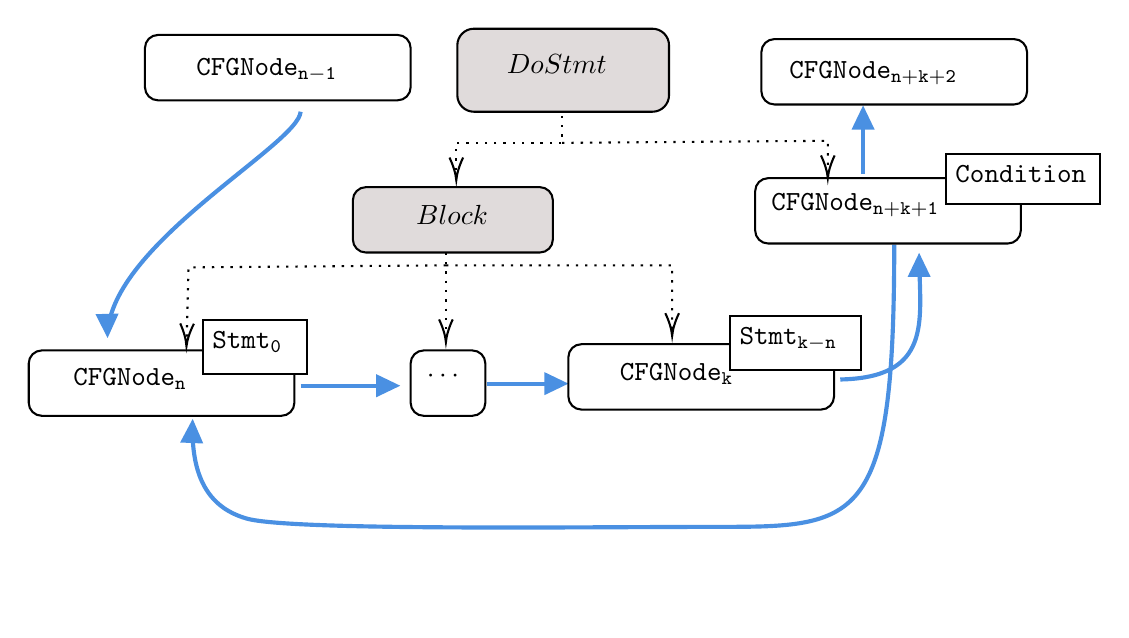
\begin{tikzpicture}[x=0.75pt,y=0.75pt,yscale=-1,xscale=1]
%uncomment if require: \path (0,607); %set diagram left start at 0, and has height of 607

%Rounded Rect [id:dp4103371580938808]
\draw  [color={rgb, 255:red, 0; green, 0; blue, 0 }  ,draw opacity=1 ][fill={rgb, 255:red, 224; green, 219; blue, 219 }  ,fill opacity=1 ] (502.5,104) .. controls (502.5,99.58) and (506.08,96) .. (510.5,96) -- (596.5,96) .. controls (600.92,96) and (604.5,99.58) .. (604.5,104) -- (604.5,128) .. controls (604.5,132.42) and (600.92,136) .. (596.5,136) -- (510.5,136) .. controls (506.08,136) and (502.5,132.42) .. (502.5,128) -- cycle ;
%Rounded Rect [id:dp7186258831078288]
\draw   (352,105.3) .. controls (352,101.82) and (354.82,99) .. (358.3,99) -- (473.7,99) .. controls (477.18,99) and (480,101.82) .. (480,105.3) -- (480,124.2) .. controls (480,127.68) and (477.18,130.5) .. (473.7,130.5) -- (358.3,130.5) .. controls (354.82,130.5) and (352,127.68) .. (352,124.2) -- cycle ;
%Curve Lines [id:da5255003767655927]
\draw [color={rgb, 255:red, 74; green, 144; blue, 226 }  ,draw opacity=1 ][line width=1.5]    (427,136) .. controls (426.03,151.52) and (338.5,198.09) .. (334.16,241.03) ;
\draw [shift={(334,245)}, rotate = 268.7] [fill={rgb, 255:red, 74; green, 144; blue, 226 }  ,fill opacity=1 ][line width=0.08]  [draw opacity=0] (11.61,-5.58) -- (0,0) -- (11.61,5.58) -- cycle    ;
%Curve Lines [id:da7123104582514019]
\draw [color={rgb, 255:red, 74; green, 144; blue, 226 }  ,draw opacity=1 ][line width=1.5]    (713,200) .. controls (713,333) and (697,336) .. (631,336) .. controls (565,336) and (422,338) .. (401,332) .. controls (381.16,326.33) and (374.71,309.94) .. (374.9,287.9) ;
\draw [shift={(375,284)}, rotate = 452.39] [fill={rgb, 255:red, 74; green, 144; blue, 226 }  ,fill opacity=1 ][line width=0.08]  [draw opacity=0] (11.61,-5.58) -- (0,0) -- (11.61,5.58) -- cycle    ;
%Curve Lines [id:da25467631423079007]
\draw [color={rgb, 255:red, 74; green, 144; blue, 226 }  ,draw opacity=1 ][line width=1.5]    (725.04,208.17) .. controls (725.61,237.55) and (730.93,264.05) .. (687,265) ;
\draw [shift={(725,204)}, rotate = 90] [fill={rgb, 255:red, 74; green, 144; blue, 226 }  ,fill opacity=1 ][line width=0.08]  [draw opacity=0] (11.61,-5.58) -- (0,0) -- (11.61,5.58) -- cycle    ;
%Rounded Rect [id:dp9303397570251196]
\draw  [fill={rgb, 255:red, 224; green, 219; blue, 219 }  ,fill opacity=1 ] (452.17,178.63) .. controls (452.17,175.15) and (454.99,172.33) .. (458.47,172.33) -- (542.23,172.33) .. controls (545.71,172.33) and (548.53,175.15) .. (548.53,178.63) -- (548.53,197.53) .. controls (548.53,201.01) and (545.71,203.83) .. (542.23,203.83) -- (458.47,203.83) .. controls (454.99,203.83) and (452.17,201.01) .. (452.17,197.53) -- cycle ;
%Straight Lines [id:da5458056196073965]
\draw [color={rgb, 255:red, 74; green, 144; blue, 226 }  ,draw opacity=1 ][line width=1.5]    (427,268) -- (471,268) ;
\draw [shift={(475,268)}, rotate = 180] [fill={rgb, 255:red, 74; green, 144; blue, 226 }  ,fill opacity=1 ][line width=0.08]  [draw opacity=0] (11.61,-5.58) -- (0,0) -- (11.61,5.58) -- cycle    ;
%Straight Lines [id:da1567518694917287]
\draw [color={rgb, 255:red, 74; green, 144; blue, 226 }  ,draw opacity=1 ][line width=1.5]    (517,267) -- (552,267) ;
\draw [shift={(556,267)}, rotate = 180] [fill={rgb, 255:red, 74; green, 144; blue, 226 }  ,fill opacity=1 ][line width=0.08]  [draw opacity=0] (11.61,-5.58) -- (0,0) -- (11.61,5.58) -- cycle    ;
%Straight Lines [id:da23667241111262138]
\draw [color={rgb, 255:red, 74; green, 144; blue, 226 }  ,draw opacity=1 ][line width=1.5]    (698,166) -- (698,137) ;
\draw [shift={(698,133)}, rotate = 450] [fill={rgb, 255:red, 74; green, 144; blue, 226 }  ,fill opacity=1 ][line width=0.08]  [draw opacity=0] (11.61,-5.58) -- (0,0) -- (11.61,5.58) -- cycle    ;
%Rounded Rect [id:dp9545385553768504]
\draw   (296,257.3) .. controls (296,253.82) and (298.82,251) .. (302.3,251) -- (417.7,251) .. controls (421.18,251) and (424,253.82) .. (424,257.3) -- (424,276.2) .. controls (424,279.68) and (421.18,282.5) .. (417.7,282.5) -- (302.3,282.5) .. controls (298.82,282.5) and (296,279.68) .. (296,276.2) -- cycle ;
%Rounded Rect [id:dp4665296267695891]
\draw   (480,257.3) .. controls (480,253.82) and (482.82,251) .. (486.3,251) -- (509.7,251) .. controls (513.18,251) and (516,253.82) .. (516,257.3) -- (516,276.2) .. controls (516,279.68) and (513.18,282.5) .. (509.7,282.5) -- (486.3,282.5) .. controls (482.82,282.5) and (480,279.68) .. (480,276.2) -- cycle ;
%Rounded Rect [id:dp31005795669558567]
\draw   (556,254.3) .. controls (556,250.82) and (558.82,248) .. (562.3,248) -- (677.7,248) .. controls (681.18,248) and (684,250.82) .. (684,254.3) -- (684,273.2) .. controls (684,276.68) and (681.18,279.5) .. (677.7,279.5) -- (562.3,279.5) .. controls (558.82,279.5) and (556,276.68) .. (556,273.2) -- cycle ;
%Rounded Rect [id:dp20286707122304926]
\draw   (646,174.3) .. controls (646,170.82) and (648.82,168) .. (652.3,168) -- (767.7,168) .. controls (771.18,168) and (774,170.82) .. (774,174.3) -- (774,193.2) .. controls (774,196.68) and (771.18,199.5) .. (767.7,199.5) -- (652.3,199.5) .. controls (648.82,199.5) and (646,196.68) .. (646,193.2) -- cycle ;
%Rounded Rect [id:dp34866856286152814]
\draw   (649,107.3) .. controls (649,103.82) and (651.82,101) .. (655.3,101) -- (770.7,101) .. controls (774.18,101) and (777,103.82) .. (777,107.3) -- (777,126.2) .. controls (777,129.68) and (774.18,132.5) .. (770.7,132.5) -- (655.3,132.5) .. controls (651.82,132.5) and (649,129.68) .. (649,126.2) -- cycle ;
%Straight Lines [id:da5919120314726174]
\draw  [dash pattern={on 0.84pt off 2.51pt}]  (497.05,210.01) -- (373,211) -- (372.05,247) ;
\draw [shift={(372,249)}, rotate = 271.51] [color={rgb, 255:red, 0; green, 0; blue, 0 }  ][line width=0.75]    (10.93,-3.29) .. controls (6.95,-1.4) and (3.31,-0.3) .. (0,0) .. controls (3.31,0.3) and (6.95,1.4) .. (10.93,3.29)   ;
%Straight Lines [id:da83242619742772]
\draw  [dash pattern={on 0.84pt off 2.51pt}]  (497.05,210.01) -- (606,210) -- (606,242) ;
\draw [shift={(606,244)}, rotate = 270] [color={rgb, 255:red, 0; green, 0; blue, 0 }  ][line width=0.75]    (10.93,-3.29) .. controls (6.95,-1.4) and (3.31,-0.3) .. (0,0) .. controls (3.31,0.3) and (6.95,1.4) .. (10.93,3.29)   ;
%Straight Lines [id:da23877345260011285]
\draw  [dash pattern={on 0.84pt off 2.51pt}]  (497,204) -- (497,245) ;
\draw [shift={(497,247)}, rotate = 270] [color={rgb, 255:red, 0; green, 0; blue, 0 }  ][line width=0.75]    (10.93,-3.29) .. controls (6.95,-1.4) and (3.31,-0.3) .. (0,0) .. controls (3.31,0.3) and (6.95,1.4) .. (10.93,3.29)   ;
%Straight Lines [id:da6580782336510713]
\draw  [dash pattern={on 0.84pt off 2.51pt}]  (553,138) -- (553,151) -- (502,151) -- (502,167) ;
\draw [shift={(502,169)}, rotate = 270] [color={rgb, 255:red, 0; green, 0; blue, 0 }  ][line width=0.75]    (10.93,-3.29) .. controls (6.95,-1.4) and (3.31,-0.3) .. (0,0) .. controls (3.31,0.3) and (6.95,1.4) .. (10.93,3.29)   ;
%Straight Lines [id:da6027446043982454]
\draw  [dash pattern={on 0.84pt off 2.51pt}]  (553,151) -- (681,150) -- (681,166) ;
\draw [shift={(681,168)}, rotate = 270] [color={rgb, 255:red, 0; green, 0; blue, 0 }  ][line width=0.75]    (10.93,-3.29) .. controls (6.95,-1.4) and (3.31,-0.3) .. (0,0) .. controls (3.31,0.3) and (6.95,1.4) .. (10.93,3.29)   ;

% Text Node
\draw (524.83,107) node [anchor=north west][inner sep=0.75pt]    {$DoStmt$};
% Text Node
\draw (375.3,109) node [anchor=north west][inner sep=0.75pt]    {$\mathtt{CFGNode_{n-1}}$};
% Text Node
\draw (661,110.3) node [anchor=north west][inner sep=0.75pt]    {$\mathtt{CFGNode_{n+k+2}}$};
% Text Node
\draw (652.3,174) node [anchor=north west][inner sep=0.75pt]    {$\mathtt{CFGNode_{n+k+1}}$};
% Text Node
\draw (481.17,179.63) node [anchor=north west][inner sep=0.75pt]    {$Block$};
% Text Node
\draw (316,258.3) node [anchor=north west][inner sep=0.75pt]    {$\mathtt{CFGNode_{n}}$};
% Text Node
\draw (486.3,259) node [anchor=north west][inner sep=0.75pt]    {$\cdots $};
% Text Node
\draw (579.3,256) node [anchor=north west][inner sep=0.75pt]    {$\mathtt{CFGNode_{k}}$};
% Text Node
\draw (504.17,373.63) node [anchor=north west][inner sep=0.75pt]    {$$};
% Text Node
\draw  [fill={rgb, 255:red, 255; green, 255; blue, 255 }  ,fill opacity=1 ]  (380,236.3) -- (430,236.3) -- (430,262.3) -- (380,262.3) -- cycle  ;
\draw (383,240.3) node [anchor=north west][inner sep=0.75pt]    {$\mathtt{Stmt_{0}}$};
% Text Node
\draw  [fill={rgb, 255:red, 255; green, 255; blue, 255 }  ,fill opacity=1 ]  (634,234.3) -- (697,234.3) -- (697,260.3) -- (634,260.3) -- cycle  ;
\draw (637,238.3) node [anchor=north west][inner sep=0.75pt]    {$\mathtt{Stmt_{k-n}}$};
% Text Node
\draw  [fill={rgb, 255:red, 255; green, 255; blue, 255 }  ,fill opacity=1 ]  (738,156.3) -- (812,156.3) -- (812,180.3) -- (738,180.3) -- cycle  ;
\draw (741,160.3) node [anchor=north west][inner sep=0.75pt]    {$\mathtt{Condition}$};


\end{tikzpicture}

%	        }
%	\end{subfigure}
%\caption{Overridden equations by \astnode{DoStmt}.}
%\label{fig:DoWhileExample}
%\end{figure}

%%EXAMPLE: ForStmt

As an example of the flexibility of \intracfg, consider the Java \astnode{ForStmt}, which is composed of variable initialisation, termination condition, post-iteration instruction, and loop body.
The {\CFG} should include a loop over these components.
However, it is legal to omit all the components, i.e., to write: `\code{for ( ; ; ) \{\}}'.
The condition is implicitly \code{true} in this case, resulting in an infinite loop.
To construct a correct {\CFG}, we still need a node to loop over; we therefore opt to reify this implicit condition.
We construct an instance of the boolean literal \code{true} as the HOA $\Ahoa{implC}$.
Figure~\ref{fig:ForStmt} shows how the $\Asyn{firstNodes}$ attribute then uses \Ahoa{implC} only if both the initialisation statements and the condition are missing.

%An example of flexibility of the framework is the implementation of the \astnode{ForStmt}.
%A standard \astnode{ForStmt} is composed by variables initialisation, termination condition, and
%the post-iteration instruction.
%A CFG of a \astnode{ForStmt} should include the expressions
%and statements in the order just indicated.
%Nevertheless, the Java Language Specification
%allows to omit all the components in the \astnode{ForStmt} and having a statement of the type
%\code{`for ( ; ; ) \{\}'}.
\begin{figure}
\hspace{-0.5cm}
 \scalebox{0.55}{
 	

% Pattern Info

\tikzset{
pattern size/.store in=\mcSize,
pattern size = 5pt,
pattern thickness/.store in=\mcThickness,
pattern thickness = 0.3pt,
pattern radius/.store in=\mcRadius,
pattern radius = 1pt}
\makeatletter
\pgfutil@ifundefined{pgf@pattern@name@_tvnte2zyq}{
\pgfdeclarepatternformonly[\mcThickness,\mcSize]{_tvnte2zyq}
{\pgfqpoint{0pt}{-\mcThickness}}
{\pgfpoint{\mcSize}{\mcSize}}
{\pgfpoint{\mcSize}{\mcSize}}
{
\pgfsetcolor{\tikz@pattern@color}
\pgfsetlinewidth{\mcThickness}
\pgfpathmoveto{\pgfqpoint{0pt}{\mcSize}}
\pgfpathlineto{\pgfpoint{\mcSize+\mcThickness}{-\mcThickness}}
\pgfusepath{stroke}
}}
\makeatother
\tikzset{every picture/.style={line width=0.75pt}} %set default line width to 0.75pt
\newsavebox\forbox
\begin{lrbox}{\forbox}
\begin{tikzpicture}
    \begin{class2}[text width=7.3cm]{ForStmt}{\astnode{ForStmt} ::= init:\astnode{Stmt}$^*$ c:\astnode{Expr} ... b:\astnode{Block}}{0, 0}
      \attribute{implements \astnode{CFGSupport}}
      \attribute{\Ahoa{implC} : \astnode{BooleanLiteral}}
      \operation{\Ahoa{implC} = new \astnode{BooleanLiteral}(true)}
      \operation{\Asyn{firstNodes} = if $\lnot$init.empty then init$_0$.\Asyn{firstNodes}}
      \operation{\hspace*{2em}elif $\lnot$c.empty then c.\Asyn{firstNodes}}
      \operation{\hspace*{2em}else \Ahoa{implC}.\Asyn{firstNodes}}
    \end{class2}
\end{tikzpicture}
\end{lrbox}
\begin{tikzpicture}[x=0.75pt,y=0.75pt,yscale=-1,xscale=1]
%uncomment if require: \path (0,1137); %set diagram left start at 0, and has height of 1137

%Rounded Rect [id:dp5100032256137063]
\draw  [fill={rgb, 255:red, 119; green, 119; blue, 119 }  ,fill opacity=1 ] (59.42,13.35) .. controls (59.42,9.84) and (62.27,7) .. (65.78,7) -- (171.95,7) .. controls (175.45,7) and (178.3,9.84) .. (178.3,13.35) -- (178.3,32.41) .. controls (178.3,35.92) and (175.45,38.77) .. (171.95,38.77) -- (65.78,38.77) .. controls (62.27,38.77) and (59.42,35.92) .. (59.42,32.41) -- cycle ;
%Rounded Rect [id:dp8990507974388595]
\draw  [dash pattern={on 4.5pt off 4.5pt}] (-0.51,75.88) .. controls (-0.51,72.37) and (2.33,69.52) .. (5.84,69.52) -- (57.03,69.52) .. controls (60.54,69.52) and (63.39,72.37) .. (63.39,75.88) -- (63.39,94.94) .. controls (63.39,98.44) and (60.54,101.29) .. (57.03,101.29) -- (5.84,101.29) .. controls (2.33,101.29) and (-0.51,98.44) .. (-0.51,94.94) -- cycle ;
%Rounded Rect [id:dp5847303802782542]
\draw  [dash pattern={on 4.5pt off 4.5pt}] (177.8,74.87) .. controls (177.8,71.36) and (180.65,68.51) .. (184.16,68.51) -- (235.35,68.51) .. controls (238.86,68.51) and (241.7,71.36) .. (241.7,74.87) -- (241.7,93.93) .. controls (241.7,97.44) and (238.86,100.28) .. (235.35,100.28) -- (184.16,100.28) .. controls (180.65,100.28) and (177.8,97.44) .. (177.8,93.93) -- cycle ;
%Straight Lines [id:da7901136535206377]
\draw  [dash pattern={on 0.84pt off 2.51pt}]  (115.89,39.27) -- (115.94,50.38) -- (67.22,69.79) ;
\draw [shift={(65.37,70.53)}, rotate = 338.27] [fill={rgb, 255:red, 0; green, 0; blue, 0 }  ][line width=0.08]  [draw opacity=0] (12,-3) -- (0,0) -- (12,3) -- cycle    ;
%Straight Lines [id:da1592958150755811]
\draw  [dash pattern={on 0.84pt off 2.51pt}]  (115.89,39.27) -- (115.94,50.38) -- (170.78,68.23) ;
\draw [shift={(172.69,68.85)}, rotate = 198.03] [fill={rgb, 255:red, 0; green, 0; blue, 0 }  ][line width=0.08]  [draw opacity=0] (12,-3) -- (0,0) -- (12,3) -- cycle    ;
%Rounded Rect [id:dp15255617186816406]
\draw  [fill={rgb, 255:red, 224; green, 219; blue, 219 }  ,fill opacity=1 ] (68.92,107.14) .. controls (68.92,103.63) and (71.76,100.78) .. (75.27,100.78) -- (158.02,100.78) .. controls (161.53,100.78) and (164.38,103.63) .. (164.38,107.14) -- (164.38,126.2) .. controls (164.38,129.71) and (161.53,132.55) .. (158.02,132.55) -- (75.27,132.55) .. controls (71.76,132.55) and (68.92,129.71) .. (68.92,126.2) -- cycle ;
%Straight Lines [id:da4530260362500649]
\draw  [dash pattern={on 0.84pt off 2.51pt}]  (115.89,133.05) -- (116.83,171.39) ;
\draw [shift={(116.88,173.39)}, rotate = 268.59000000000003] [fill={rgb, 255:red, 0; green, 0; blue, 0 }  ][line width=0.08]  [draw opacity=0] (12,-3) -- (0,0) -- (12,3) -- cycle    ;
%Straight Lines [id:da008572923107979857]
\draw  [dash pattern={on 0.84pt off 2.51pt}]  (115.89,39.27) -- (115.89,95.76) ;
\draw [shift={(115.89,97.76)}, rotate = 270] [fill={rgb, 255:red, 0; green, 0; blue, 0 }  ][line width=0.08]  [draw opacity=0] (12,-3) -- (0,0) -- (12,3) -- cycle    ;
%Straight Lines [id:da48612698188167747]
\draw [color={rgb, 255:red, 74; green, 144; blue, 226 }  ,draw opacity=1 ][line width=1.5]    (47.21,280.9) -- (27.43,280.9) -- (27.43,103.42) ;
\draw [shift={(51.21,280.9)}, rotate = 180] [fill={rgb, 255:red, 74; green, 144; blue, 226 }  ,fill opacity=1 ][line width=0.08]  [draw opacity=0] (11.61,-5.58) -- (0,0) -- (11.61,5.58) -- cycle    ;
%Rounded Rect [id:dp33150746930836394]
\draw  [fill={rgb, 255:red, 224; green, 219; blue, 219 }  ,fill opacity=1 ] (70.9,183.78) .. controls (70.9,180.27) and (73.74,177.43) .. (77.25,177.43) -- (160,177.43) .. controls (163.51,177.43) and (166.36,180.27) .. (166.36,183.78) -- (166.36,202.84) .. controls (166.36,206.35) and (163.51,209.19) .. (160,209.19) -- (77.25,209.19) .. controls (73.74,209.19) and (70.9,206.35) .. (70.9,202.84) -- cycle ;
%Rounded Rect [id:dp034528485502401174]
\draw  [dash pattern={on 4.5pt off 4.5pt}] (55.46,267.38) .. controls (55.46,261.7) and (60.07,257.09) .. (65.75,257.09) -- (174.95,257.09) .. controls (180.63,257.09) and (185.23,261.7) .. (185.23,267.38) -- (185.23,298.24) .. controls (185.23,303.92) and (180.63,308.52) .. (174.95,308.52) -- (65.75,308.52) .. controls (60.07,308.52) and (55.46,303.92) .. (55.46,298.24) -- cycle ;
%Straight Lines [id:da25032488377016593]
\draw  [dash pattern={on 0.84pt off 2.51pt}]  (116.88,211.71) -- (116.88,248.03) ;
\draw [shift={(116.88,250.03)}, rotate = 270] [fill={rgb, 255:red, 0; green, 0; blue, 0 }  ][line width=0.08]  [draw opacity=0] (12,-3) -- (0,0) -- (12,3) -- cycle    ;
%Curve Lines [id:da9247423588036267]
\draw [color={rgb, 255:red, 74; green, 144; blue, 226 }  ,draw opacity=1 ][line width=1.5]    (83.2,312.56) .. controls (54.07,362.96) and (135.31,362.03) .. (105.01,316.41) ;
\draw [shift={(103.01,313.57)}, rotate = 413.62] [fill={rgb, 255:red, 74; green, 144; blue, 226 }  ,fill opacity=1 ][line width=0.08]  [draw opacity=0] (11.61,-5.58) -- (0,0) -- (11.61,5.58) -- cycle    ;
%Straight Lines [id:da48274161194562804]
\draw  [dash pattern={on 0.84pt off 2.51pt}]  (117.15,220.76) -- (245.87,221.2) -- (245.87,247.3) ;
\draw [shift={(245.87,249.3)}, rotate = 270] [fill={rgb, 255:red, 0; green, 0; blue, 0 }  ][line width=0.08]  [draw opacity=0] (12,-3) -- (0,0) -- (12,3) -- cycle    ;
%Rounded Rect [id:dp047161589513216584]
\draw  [fill={rgb, 255:red, 224; green, 219; blue, 219 }  ,fill opacity=1 ] (214.68,258.4) .. controls (214.68,254.9) and (217.52,252.05) .. (221.03,252.05) -- (265.15,252.05) .. controls (268.66,252.05) and (271.5,254.9) .. (271.5,258.4) -- (271.5,277.46) .. controls (271.5,280.97) and (268.66,283.82) .. (265.15,283.82) -- (221.03,283.82) .. controls (217.52,283.82) and (214.68,280.97) .. (214.68,277.46) -- cycle ;
%Straight Lines [id:da48225680942513005]
\draw [color={rgb, 255:red, 74; green, 144; blue, 226 }  ,draw opacity=1 ][line width=1.5]    (185.23,267.38) -- (205.62,267.39) -- (205.62,106.63) ;
\draw [shift={(205.62,102.63)}, rotate = 450] [fill={rgb, 255:red, 74; green, 144; blue, 226 }  ,fill opacity=1 ][line width=0.08]  [draw opacity=0] (11.61,-5.58) -- (0,0) -- (11.61,5.58) -- cycle    ;
%Curve Lines [id:da7422459460743117]
\draw [color={rgb, 255:red, 126; green, 211; blue, 33 }  ,draw opacity=1 ][line width=1.5]  [dash pattern={on 5.63pt off 4.5pt}]  (68.4,118.13) .. controls (27.02,164.89) and (30.44,221.32) .. (54.19,254.12) ;
\draw [shift={(56.45,257.09)}, rotate = 231.4] [fill={rgb, 255:red, 126; green, 211; blue, 33 }  ,fill opacity=1 ][line width=0.08]  [draw opacity=0] (11.61,-5.58) -- (0,0) -- (11.61,5.58) -- cycle    ;
%Curve Lines [id:da009130105523222576]
\draw [color={rgb, 255:red, 126; green, 211; blue, 33 }  ,draw opacity=1 ][line width=1.5]  [dash pattern={on 5.63pt off 4.5pt}]  (69.89,189.83) .. controls (44.54,210.7) and (30.69,224.82) .. (56.45,257.09) ;
%Curve Lines [id:da18611103922131644]
\draw [color={rgb, 255:red, 126; green, 211; blue, 33 }  ,draw opacity=1 ][line width=1.5]  [dash pattern={on 5.63pt off 4.5pt}]  (133.72,312.56) .. controls (104.6,362.96) and (185.83,362.03) .. (155.53,316.41) ;
\draw [shift={(153.53,313.57)}, rotate = 413.62] [fill={rgb, 255:red, 126; green, 211; blue, 33 }  ,fill opacity=1 ][line width=0.08]  [draw opacity=0] (11.61,-5.58) -- (0,0) -- (11.61,5.58) -- cycle    ;
%Curve Lines [id:da7711201281153591]
\draw [color={rgb, 255:red, 126; green, 211; blue, 33 }  ,draw opacity=1 ][line width=1.5]  [dash pattern={on 5.63pt off 4.5pt}]  (239.19,285.88) .. controls (239.19,295.19) and (237.48,291.62) .. (191.65,291.88) ;
\draw [shift={(188.03,291.91)}, rotate = 359.44] [fill={rgb, 255:red, 126; green, 211; blue, 33 }  ,fill opacity=1 ][line width=0.08]  [draw opacity=0] (11.61,-5.58) -- (0,0) -- (11.61,5.58) -- cycle    ;
%Curve Lines [id:da05649695805427568]
\draw [color={rgb, 255:red, 126; green, 211; blue, 33 }  ,draw opacity=1 ][line width=1.5]  [dash pattern={on 5.63pt off 4.5pt}]  (5.73,101.29) .. controls (-21.4,135.17) and (36.26,130.97) .. (16.95,104.65) ;
\draw [shift={(14.54,101.7)}, rotate = 408.02] [fill={rgb, 255:red, 126; green, 211; blue, 33 }  ,fill opacity=1 ][line width=0.08]  [draw opacity=0] (11.61,-5.58) -- (0,0) -- (11.61,5.58) -- cycle    ;
%Curve Lines [id:da38645058437295565]
\draw [color={rgb, 255:red, 126; green, 211; blue, 33 }  ,draw opacity=1 ][line width=1.5]  [dash pattern={on 5.63pt off 4.5pt}]  (226.65,99.87) .. controls (199.52,133.75) and (257.18,129.55) .. (237.87,103.23) ;
\draw [shift={(235.46,100.28)}, rotate = 408.02] [fill={rgb, 255:red, 126; green, 211; blue, 33 }  ,fill opacity=1 ][line width=0.08]  [draw opacity=0] (11.61,-5.58) -- (0,0) -- (11.61,5.58) -- cycle    ;
%Shape: Rectangle [id:dp18462636620367567]
\draw   (282,264.86) -- (509.5,264.86) -- (509.5,345.5) -- (282,345.5) -- cycle ;
%Rounded Rect [id:dp21294641657728508]
\draw  [fill={rgb, 255:red, 255; green, 255; blue, 255 }  ,fill opacity=1 ] (398.93,271.56) .. controls (398.93,270.06) and (400.15,268.84) .. (401.66,268.84) -- (409.83,268.84) .. controls (411.34,268.84) and (412.56,270.06) .. (412.56,271.56) -- (412.56,282) .. controls (412.56,283.5) and (411.34,284.72) .. (409.83,284.72) -- (401.66,284.72) .. controls (400.15,284.72) and (398.93,283.5) .. (398.93,282) -- cycle ;
%Rounded Rect [id:dp5648235410650739]
\draw  [fill={rgb, 255:red, 119; green, 119; blue, 119 }  ,fill opacity=1 ] (288.53,291.22) .. controls (288.53,289.83) and (289.66,288.69) .. (291.06,288.69) -- (298.66,288.69) .. controls (300.05,288.69) and (301.19,289.83) .. (301.19,291.22) -- (301.19,301.05) .. controls (301.19,302.45) and (300.05,303.59) .. (298.66,303.59) -- (291.06,303.59) .. controls (289.66,303.59) and (288.53,302.45) .. (288.53,301.05) -- cycle ;
%Rounded Rect [id:dp37060502353713864]
\draw  [fill={rgb, 255:red, 224; green, 219; blue, 219 }  ,fill opacity=1 ] (398.93,292.41) .. controls (398.93,290.91) and (400.15,289.69) .. (401.66,289.69) -- (409.83,289.69) .. controls (411.34,289.69) and (412.56,290.91) .. (412.56,292.41) -- (412.56,302.85) .. controls (412.56,304.35) and (411.34,305.57) .. (409.83,305.57) -- (401.66,305.57) .. controls (400.15,305.57) and (398.93,304.35) .. (398.93,302.85) -- cycle ;
%Rounded Rect [id:dp09724209068955114]
\draw  [fill={rgb, 255:red, 224; green, 219; blue, 219 }  ,fill opacity=1 ] (294.95,269.07) .. controls (294.95,268.39) and (295.5,267.84) .. (296.18,267.84) -- (299.85,267.84) .. controls (300.53,267.84) and (301.08,268.39) .. (301.08,269.07) -- (301.08,273.65) .. controls (301.08,274.32) and (300.53,274.87) .. (299.85,274.87) -- (296.18,274.87) .. controls (295.5,274.87) and (294.95,274.32) .. (294.95,273.65) -- cycle ;
%Rounded Rect [id:dp0017317963746376064]
\draw  [pattern=_tvnte2zyq,pattern size=2.8499999999999996pt,pattern thickness=0.75pt,pattern radius=0pt, pattern color={rgb, 255:red, 0; green, 0; blue, 0}] (294.95,276.02) .. controls (294.95,275.34) and (295.5,274.79) .. (296.18,274.79) -- (299.85,274.79) .. controls (300.53,274.79) and (301.08,275.34) .. (301.08,276.02) -- (301.08,280.6) .. controls (301.08,281.27) and (300.53,281.82) .. (299.85,281.82) -- (296.18,281.82) .. controls (295.5,281.82) and (294.95,281.27) .. (294.95,280.6) -- cycle ;
%Rounded Rect [id:dp12164830585442543]
\draw  [fill={rgb, 255:red, 255; green, 255; blue, 255 }  ,fill opacity=1 ][dash pattern={on 0.84pt off 2.51pt}] (288.62,310.55) .. controls (288.62,309.04) and (289.83,307.82) .. (291.34,307.82) -- (299.51,307.82) .. controls (301.02,307.82) and (302.24,309.04) .. (302.24,310.55) -- (302.24,320.98) .. controls (302.24,322.49) and (301.02,323.71) .. (299.51,323.71) -- (291.34,323.71) .. controls (289.83,323.71) and (288.62,322.49) .. (288.62,320.98) -- cycle ;
%Straight Lines [id:da7218140703896597]
\draw [color={rgb, 255:red, 126; green, 211; blue, 33 }  ,draw opacity=1 ][line width=1.5]  [dash pattern={on 5.63pt off 4.5pt}]  (285.02,337.51) -- (307.73,337.59) ;
\draw [shift={(311.73,337.61)}, rotate = 180.21] [fill={rgb, 255:red, 126; green, 211; blue, 33 }  ,fill opacity=1 ][line width=0.08]  [draw opacity=0] (11.61,-5.58) -- (0,0) -- (11.61,5.58) -- cycle    ;
%Rounded Rect [id:dp5560182938693506]
\draw  [fill={rgb, 255:red, 255; green, 255; blue, 255 }  ,fill opacity=1 ][dash pattern={on 0.84pt off 2.51pt}] (287.87,269.07) .. controls (287.87,268.39) and (288.42,267.84) .. (289.09,267.84) -- (292.77,267.84) .. controls (293.44,267.84) and (293.99,268.39) .. (293.99,269.07) -- (293.99,273.65) .. controls (293.99,274.32) and (293.44,274.87) .. (292.77,274.87) -- (289.09,274.87) .. controls (288.42,274.87) and (287.87,274.32) .. (287.87,273.65) -- cycle ;
%Rounded Rect [id:dp6782076153242217]
\draw  [fill={rgb, 255:red, 119; green, 119; blue, 119 }  ,fill opacity=1 ] (287.9,276.02) .. controls (287.9,275.34) and (288.44,274.79) .. (289.12,274.79) -- (292.79,274.79) .. controls (293.47,274.79) and (294.02,275.34) .. (294.02,276.02) -- (294.02,280.6) .. controls (294.02,281.27) and (293.47,281.82) .. (292.79,281.82) -- (289.12,281.82) .. controls (288.44,281.82) and (287.9,281.27) .. (287.9,280.6) -- cycle ;
%Straight Lines [id:da5185875420103297]
\draw [color={rgb, 255:red, 74; green, 144; blue, 226 }  ,draw opacity=1 ][line width=1.5]    (398.59,319.67) -- (416.3,319.75) ;
\draw [shift={(420.3,319.77)}, rotate = 180.26] [fill={rgb, 255:red, 74; green, 144; blue, 226 }  ,fill opacity=1 ][line width=0.08]  [draw opacity=0] (11.61,-5.58) -- (0,0) -- (11.61,5.58) -- cycle    ;
%Straight Lines [id:da5761225056777026]
\draw    (275,8) -- (275.5,343.5) ;

% Text Node
\draw (75.2,15.54) node [anchor=north west][inner sep=0.75pt]  [color={rgb, 255:red, 255; green, 255; blue, 255 }  ,opacity=1 ]  {$\mathtt{MethodDecl}$};
% Text Node
\draw (10.02,78.06) node [anchor=north west][inner sep=0.75pt]    {$\mathtt{Entry}$};
% Text Node
\draw (196.78,78.81) node [anchor=north west][inner sep=0.75pt]    {$\mathtt{Exit}$};
% Text Node
\draw (97.21,109.32) node [anchor=north west][inner sep=0.75pt]    {$\mathtt{Block}$};
% Text Node
\draw (91.5,186.6) node [anchor=north west][inner sep=0.75pt]    {$\mathtt{ForStmt}$};
% Text Node
\draw (36.47,336.84) node [anchor=north west][inner sep=0.75pt]   [align=left] {\begin{minipage}[lt]{25.57pt}\setlength\topsep{0pt}
\begin{center}
{\fontfamily{pcr}\selectfont {\small True}}
\end{center}

\end{minipage}};
% Text Node
\draw (63.49,265.58) node [anchor=north west][inner sep=0.75pt]    {$\mathtt{BooleanLiteral}$};
% Text Node
\draw (84.14,285.8) node [anchor=north west][inner sep=0.75pt]    {$\mathtt{< true >}$};
% Text Node
\draw (222.17,260.59) node [anchor=north west][inner sep=0.75pt]    {$\mathtt{Block}$};
% Text Node
\draw (190.3,203.54) node [anchor=north west][inner sep=0.75pt]  [rotate=-269.48] [align=left] {\begin{minipage}[lt]{31.29pt}\setlength\topsep{0pt}
\begin{center}
{\fontfamily{pcr}\selectfont {\small False}}
\end{center}

\end{minipage}};
% Text Node
\draw (310,289.37) node [anchor=north west][inner sep=0.75pt]    {$\mathtt{CFGRoot}$};
% Text Node
\draw (420,269.51) node [anchor=north west][inner sep=0.75pt]    {$\mathtt{CFGNode}$};
% Text Node
\draw (420,292) node [anchor=north west][inner sep=0.75pt]    {$\mathtt{CFGSupport}$};
% Text Node
\draw (310,268.52) node [anchor=north west][inner sep=0.75pt]    {$\mathtt{AST\ node}$};
% Text Node
\draw (285.22,247.93) node [anchor=north west][inner sep=0.75pt]   [align=left] {\textit{Legend}};
% Text Node
\draw (310,309.52) node [anchor=north west][inner sep=0.75pt]    {$\mathtt{HOA}$};
% Text Node
\draw (317.08,331.33) node [anchor=north west][inner sep=0.75pt]    {\Asyn{firstNodes}};
% Text Node
\draw (424.47,314.49) node [anchor=north west][inner sep=0.75pt]    {\Asyn{succ}};
% Text Node
\draw (276.85,11.29) node [anchor=north west][scale=1.7]    {		   \begin{lstlisting}[language=java,frame=none]
void foo(){
  for( ; ; ){  }
}
	       \end{lstlisting}
};

% Text Node
\draw (275.00,90.0) node [anchor=north west][scale=1.15]    {
\usebox\forbox};


\end{tikzpicture}

 }
\caption{CFG for method with empty \emph{ForStmt}. The HOA \Ahoa{implC} reifies the implicit \emph{true} condition.
}
\label{fig:ForStmt}
\end{figure}
%Because there are no action nodes, the resulting CFG would completely
%exclude the AST rooted in  \astnode{ForStmt}, disallowing any analysis to detect the presence
%of a trivial infinite-loop.
%The problem occurs when the condition is omitted.
%To overcome this problem, we defined the HOA \astnode{implicitCond}, which is an instance
%of the boolean literal \code{true}.
%This HOA is instantiated and included in the CFG only
%when the termination condition is implicit.



%%EXAMPLE: EmptyStmt
Another interesting corner case is the  \astnode{EmptyStmt}.
This node represents e.g. the semicolon in the trivial block \code{\{;\}}.
The \astnode{EmptyStmt} is a \astnode{CFGSupport} node
since it does not map to a runtime action.
Since \astnode{EmptyStmt} has no children, its \Asyn{firstNodes} will be the following CFG node.
We achieve this by defining $\Asyn{firstNodes}$ as equal to \mbox{$\Ainh{nextNodes}$}, overriding the default equation from \astnode{CFGSupport}.
In this manner, the {\CFG} skips the \astnode{EmptyStmt},
and if there are occurrences of multiple \astnode{EmptyStmt}s, we skip them transitively
and link to the next concrete \astnode{CFGNode}.
The example in Figure~\ref{fig:EmptyStmt}
shows how we exclude two \astnode{EmptyStmt}s from the {\CFG} and obtain a {\CFG}
with only a single edge from method \astnode{Entry} to \astnode{Exit}.
Let us call the two \astnode{EmptyStmt}s $e_1$ and $e_2$, from left to right.
The equations give that $\astnode{Entry}.\Asyn{succ} = \astnode{Exit}$ since %\\\\
% $\astnode{Entry}.\Asyn{succ}  = \astnode{Entry}.\Ainh{nextNodes} = \astnode{Block}.\Asyn{firstNodes}$\\
% \hspace*{2em}  $= e_1.\Asyn{firstNodes} = e_1.\Ainh{nextNodes}$ \\
% \hspace*{2em}  $= e_2.\Asyn{firstNodes} = e_2.\Ainh{nextNodes}$ \\
% \hspace*{2em}  $= \astnode{Block}.\Ainh{nextNodes} = \astnode{Exit}$
\[\begin{array}{r@{\:}c@{\:}c@{\:}c@{\:}l}
\astnode{Entry}.\Asyn{succ} &=& \astnode{Entry}.\Ainh{nextNodes} &=& \astnode{Block}.\Asyn{firstNodes} \\
                            &=& e_1.\Asyn{firstNodes} &=& e_1.\Ainh{nextNodes} \\
                            &=& e_2.\Asyn{firstNodes} &=& e_2.\Ainh{nextNodes} \\
                            &=& \astnode{Block}.\Ainh{nextNodes} &=& \astnode{Exit}
  \end{array}
\]

%The \astnode{Block} now lets $e_3$ inherit
%$e_3.\Ainh{nextNodes} = \astnode{Exit}$, while $e_2$ inherits from $e_3$ via
%$e_2.\Ainh{nextNodes} = e_3.\Asyn{firstNodes}$ and $e_1$ analogously,
%$e_1.\Ainh{nextNodes} = e_2.\Asyn{firstNodes}$.
%Since \astnode{EmptyStmt} defines $n.\Asyn{firstNodes} = n.\Ainh{nextNodes}$ for all nodes $n$ that are \astnode{EmptyStmt}, we
%obtain
%\[\begin{array}{lclcl}
%    e_1.\Ainh{firstNodes} &=& e_1.\Ainh{nextNodes}\\
%                           &=& e_2.\Ainh{firstNodes}\\
%                           &=& e_2.\Ainh{nextNodes}\\
%                           &=& e_3.\Ainh{firstNodes}\\
%                           &=& e_3.\Ainh{nextNodes} &=& \astnode{Exit}
%  \end{array}
%\]

  \begin{figure}
\hspace{-0.42cm}
 \scalebox{0.6}{
 

% Pattern Info

\tikzset{
pattern size/.store in=\mcSize,
pattern size = 5pt,
pattern thickness/.store in=\mcThickness,
pattern thickness = 0.3pt,
pattern radius/.store in=\mcRadius,
pattern radius = 1pt}
\makeatletter
\pgfutil@ifundefined{pgf@pattern@name@_1ly9gcxx6}{
\pgfdeclarepatternformonly[\mcThickness,\mcSize]{_1ly9gcxx6}
{\pgfqpoint{0pt}{-\mcThickness}}
{\pgfpoint{\mcSize}{\mcSize}}
{\pgfpoint{\mcSize}{\mcSize}}
{
\pgfsetcolor{\tikz@pattern@color}
\pgfsetlinewidth{\mcThickness}
\pgfpathmoveto{\pgfqpoint{0pt}{\mcSize}}
\pgfpathlineto{\pgfpoint{\mcSize+\mcThickness}{-\mcThickness}}
\pgfusepath{stroke}
}}
\makeatother
\tikzset{every picture/.style={line width=0.75pt}} %set default line width to 0.75pt
\newsavebox\emptystmtbox
\begin{lrbox}{\emptystmtbox}
\begin{tikzpicture}
    \begin{class2}[text width=4cm]{EmptyStmt}{\astnode{EmptyStmt}}{0, 0}
      \attribute{implements \astnode{CFGSupport}}
      \operation{\Asyn{firstNodes} = \Ainh{nextNodes}}
    \end{class2}
\end{tikzpicture}
\end{lrbox}
\begin{tikzpicture}[x=0.75pt,y=0.75pt,yscale=-1,xscale=1]
%uncomment if require: \path (0,1137); %set diagram left start at 0, and has height of 1137

%Rounded Rect [id:dp9553143030411669]
\draw  [fill={rgb, 255:red, 119; green, 119; blue, 119 }  ,fill opacity=1 ] (113.97,14.81) .. controls (113.97,11.6) and (116.57,9) .. (119.79,9) -- (216.17,9) .. controls (219.38,9) and (221.98,11.6) .. (221.98,14.81) -- (221.98,32.25) .. controls (221.98,35.46) and (219.38,38.07) .. (216.17,38.07) -- (119.79,38.07) .. controls (116.57,38.07) and (113.97,35.46) .. (113.97,32.25) -- cycle ;
%Rounded Rect [id:dp3918952455814019]
\draw  [dash pattern={on 4.5pt off 4.5pt}] (59.52,72.02) .. controls (59.52,68.81) and (62.12,66.21) .. (65.33,66.21) -- (111.76,66.21) .. controls (114.97,66.21) and (117.57,68.81) .. (117.57,72.02) -- (117.57,89.47) .. controls (117.57,92.68) and (114.97,95.28) .. (111.76,95.28) -- (65.33,95.28) .. controls (62.12,95.28) and (59.52,92.68) .. (59.52,89.47) -- cycle ;
%Rounded Rect [id:dp21414115284566693]
\draw  [dash pattern={on 4.5pt off 4.5pt}] (221.53,71.1) .. controls (221.53,67.89) and (224.14,65.29) .. (227.35,65.29) -- (273.78,65.29) .. controls (276.99,65.29) and (279.59,67.89) .. (279.59,71.1) -- (279.59,88.54) .. controls (279.59,91.75) and (276.99,94.36) .. (273.78,94.36) -- (227.35,94.36) .. controls (224.14,94.36) and (221.53,91.75) .. (221.53,88.54) -- cycle ;
%Straight Lines [id:da4709337177480183]
\draw  [dash pattern={on 0.84pt off 2.51pt}]  (165.28,38.53) -- (165.32,48.69) -- (121.23,66.39) ;
\draw [shift={(119.37,67.13)}, rotate = 338.13] [fill={rgb, 255:red, 0; green, 0; blue, 0 }  ][line width=0.08]  [draw opacity=0] (12,-3) -- (0,0) -- (12,3) -- cycle    ;
%Straight Lines [id:da2935223472020221]
\draw  [dash pattern={on 0.84pt off 2.51pt}]  (165.28,38.53) -- (165.32,48.69) -- (217.97,65) ;
\draw [shift={(219.88,65.6)}, rotate = 197.21] [fill={rgb, 255:red, 0; green, 0; blue, 0 }  ][line width=0.08]  [draw opacity=0] (12,-3) -- (0,0) -- (12,3) -- cycle    ;
%Rounded Rect [id:dp135780542904527]
\draw  [fill={rgb, 255:red, 224; green, 219; blue, 219 }  ,fill opacity=1 ] (122.6,100.63) .. controls (122.6,97.42) and (125.2,94.82) .. (128.41,94.82) -- (203.52,94.82) .. controls (206.73,94.82) and (209.33,97.42) .. (209.33,100.63) -- (209.33,118.07) .. controls (209.33,121.28) and (206.73,123.88) .. (203.52,123.88) -- (128.41,123.88) .. controls (125.2,123.88) and (122.6,121.28) .. (122.6,118.07) -- cycle ;
%Straight Lines [id:da5646799262927455]
\draw  [dash pattern={on 0.84pt off 2.51pt}]  (165.28,38.53) -- (165.28,90.05) ;
\draw [shift={(165.28,92.05)}, rotate = 270] [fill={rgb, 255:red, 0; green, 0; blue, 0 }  ][line width=0.08]  [draw opacity=0] (12,-3) -- (0,0) -- (12,3) -- cycle    ;
%Straight Lines [id:da6024250973498378]
\draw [color={rgb, 255:red, 74; green, 144; blue, 226 }  ,draw opacity=1 ][line width=1.5]    (250.79,102.51) -- (250.79,139.42) -- (85.17,139.42) -- (84.9,97.23) ;
\draw [shift={(250.79,98.51)}, rotate = 90] [fill={rgb, 255:red, 74; green, 144; blue, 226 }  ,fill opacity=1 ][line width=0.08]  [draw opacity=0] (11.61,-5.58) -- (0,0) -- (11.61,5.58) -- cycle    ;
%Rounded Rect [id:dp17052492437405065]
\draw  [fill={rgb, 255:red, 224; green, 219; blue, 219 }  ,fill opacity=1 ] (18.5,188.29) .. controls (18.5,185.08) and (21.1,182.48) .. (24.31,182.48) -- (101.96,182.48) .. controls (105.17,182.48) and (107.77,185.08) .. (107.77,188.29) -- (107.77,205.73) .. controls (107.77,208.94) and (105.17,211.55) .. (101.96,211.55) -- (24.31,211.55) .. controls (21.1,211.55) and (18.5,208.94) .. (18.5,205.73) -- cycle ;
%Rounded Rect [id:dp4000967205848748]
\draw  [fill={rgb, 255:red, 224; green, 219; blue, 219 }  ,fill opacity=1 ] (236.5,188.29) .. controls (236.5,185.08) and (239.1,182.48) .. (242.31,182.48) -- (322.69,182.48) .. controls (325.9,182.48) and (328.5,185.08) .. (328.5,188.29) -- (328.5,205.73) .. controls (328.5,208.94) and (325.9,211.55) .. (322.69,211.55) -- (242.31,211.55) .. controls (239.1,211.55) and (236.5,208.94) .. (236.5,205.73) -- cycle ;
%Straight Lines [id:da3318797505997164]
\draw  [dash pattern={on 0.84pt off 2.51pt}]  (166.18,125.27) -- (166.22,135.43) -- (85.82,178.71) ;
\draw [shift={(84.06,179.66)}, rotate = 331.71000000000004] [fill={rgb, 255:red, 0; green, 0; blue, 0 }  ][line width=0.08]  [draw opacity=0] (12,-3) -- (0,0) -- (12,3) -- cycle    ;
%Straight Lines [id:da035361006569364584]
\draw  [dash pattern={on 0.84pt off 2.51pt}]  (166.18,125.27) -- (166.22,135.43) -- (248.12,179.63) ;
\draw [shift={(249.88,180.58)}, rotate = 208.36] [fill={rgb, 255:red, 0; green, 0; blue, 0 }  ][line width=0.08]  [draw opacity=0] (12,-3) -- (0,0) -- (12,3) -- cycle    ;
%Straight Lines [id:da9053529414539677]
%\draw  [dash pattern={on 0.84pt off 2.51pt}]  (166.18,125.27) -- (166.18,178.79) ;
%\draw [shift={(166.18,180.79)}, rotate = 270] [fill={rgb, 255:red, 0; green, 0; blue, 0 }  ][line width=0.08]  [draw opacity=0] (12,-3) -- (0,0) -- (12,3) -- cycle    ;
%Rounded Rect [id:dp5957216742820051]
%\draw  [fill={rgb, 255:red, 224; green, 219; blue, 219 }  ,fill opacity=1 ] (123.5,188.29) .. controls (123.5,185.08) and (126.1,182.48) .. (129.31,182.48) -- (207.67,182.48) .. controls (210.88,182.48) and (213.48,185.08) .. (213.48,188.29) -- (213.48,205.73) .. controls (213.48,208.94) and (210.88,211.55) .. (207.67,211.55) -- (129.31,211.55) .. controls (126.1,211.55) and (123.5,208.94) .. (123.5,205.73) -- cycle ;
%Shape: Rectangle [id:dp2571888827155022]
\draw   (338,149) -- (593.5,149) -- (593.5,237) -- (338,237) -- cycle ;
%Rounded Rect [id:dp8790474866569303]
\draw  [fill={rgb, 255:red, 255; green, 255; blue, 255 }  ,fill opacity=1 ] (345.49,196.92) .. controls (345.49,195.31) and (346.8,194) .. (348.41,194) -- (357.19,194) .. controls (358.8,194) and (360.11,195.31) .. (360.11,196.92) -- (360.11,207.08) .. controls (360.11,208.69) and (358.8,210) .. (357.19,210) -- (348.41,210) .. controls (346.8,210) and (345.49,208.69) .. (345.49,207.08) -- cycle ;
%Rounded Rect [id:dp1497018934664086]
\draw  [fill={rgb, 255:red, 119; green, 119; blue, 119 }  ,fill opacity=1 ] (345.01,175.72) .. controls (345.01,174.22) and (346.22,173) .. (347.72,173) -- (355.87,173) .. controls (357.37,173) and (358.59,174.22) .. (358.59,175.72) -- (358.59,185.28) .. controls (358.59,186.78) and (357.37,188) .. (355.87,188) -- (347.72,188) .. controls (346.22,188) and (345.01,186.78) .. (345.01,185.28) -- cycle ;
%Rounded Rect [id:dp045296504188673814]
\draw  [fill={rgb, 255:red, 224; green, 219; blue, 219 }  ,fill opacity=1 ] (345.49,217.92) .. controls (345.49,216.31) and (346.8,215) .. (348.41,215) -- (357.19,215) .. controls (358.8,215) and (360.11,216.31) .. (360.11,217.92) -- (360.11,228.08) .. controls (360.11,229.69) and (358.8,231) .. (357.19,231) -- (348.41,231) .. controls (346.8,231) and (345.49,229.69) .. (345.49,228.08) -- cycle ;
%Rounded Rect [id:dp5762833369010006]
\draw  [fill={rgb, 255:red, 255; green, 255; blue, 255 }  ,fill opacity=1 ][dash pattern={on 0.84pt off 2.51pt}] (470.49,157.92) .. controls (470.49,156.31) and (471.8,155) .. (473.41,155) -- (482.19,155) .. controls (483.8,155) and (485.11,156.31) .. (485.11,157.92) -- (485.11,168.08) .. controls (485.11,169.69) and (483.8,171) .. (482.19,171) -- (473.41,171) .. controls (471.8,171) and (470.49,169.69) .. (470.49,168.08) -- cycle ;
%Straight Lines [id:da019202562948454127]
\draw [color={rgb, 255:red, 126; green, 211; blue, 33 }  ,draw opacity=1 ][line width=1.5]  [dash pattern={on 5.63pt off 4.5pt}]  (465,184.9) -- (479.51,184.96) -- (487,184.98) ;
\draw [shift={(491,185)}, rotate = 180.22] [fill={rgb, 255:red, 126; green, 211; blue, 33 }  ,fill opacity=1 ][line width=0.08]  [draw opacity=0] (11.61,-5.58) -- (0,0) -- (11.61,5.58) -- cycle    ;
%Straight Lines [id:da45208513444314147]
\draw [color={rgb, 255:red, 74; green, 144; blue, 226 }  ,draw opacity=1 ][line width=1.5]    (466,206.9) -- (489,206.99) ;
\draw [shift={(493,207)}, rotate = 180.21] [fill={rgb, 255:red, 74; green, 144; blue, 226 }  ,fill opacity=1 ][line width=0.08]  [draw opacity=0] (11.61,-5.58) -- (0,0) -- (11.61,5.58) -- cycle    ;
%Curve Lines [id:da8998932683526912]
\draw [color={rgb, 255:red, 126; green, 211; blue, 33 }  ,draw opacity=1 ][line width=1.5]  [dash pattern={on 5.63pt off 4.5pt}]  (65.19,95.28) .. controls (40.66,126.12) and (92.39,122.48) .. (75.65,98.73) ;
\draw [shift={(73.19,95.66)}, rotate = 408.22] [fill={rgb, 255:red, 126; green, 211; blue, 33 }  ,fill opacity=1 ][line width=0.08]  [draw opacity=0] (11.61,-5.58) -- (0,0) -- (11.61,5.58) -- cycle    ;
%Curve Lines [id:da024105029587362936]
\draw [color={rgb, 255:red, 126; green, 211; blue, 33 }  ,draw opacity=1 ][line width=1.5]  [dash pattern={on 5.63pt off 4.5pt}]  (265.91,93.98) .. controls (241.39,124.82) and (293.12,121.18) .. (276.38,97.43) ;
\draw [shift={(273.92,94.36)}, rotate = 408.22] [fill={rgb, 255:red, 126; green, 211; blue, 33 }  ,fill opacity=1 ][line width=0.08]  [draw opacity=0] (11.61,-5.58) -- (0,0) -- (11.61,5.58) -- cycle    ;
%Curve Lines [id:da004999379060312337]
\draw [color={rgb, 255:red, 126; green, 211; blue, 33 }  ,draw opacity=1 ][line width=1.5]  [dash pattern={on 5.63pt off 4.5pt}]  (57.5,180) .. controls (73.89,160.48) and (231.69,155.83) .. (237.15,100.06) ;
\draw [shift={(237.29,96.59)}, rotate = 449.13] [fill={rgb, 255:red, 126; green, 211; blue, 33 }  ,fill opacity=1 ][line width=0.08]  [draw opacity=0] (11.61,-5.58) -- (0,0) -- (11.61,5.58) -- cycle    ;
%Curve Lines [id:da511749178474782]
%\draw [color={rgb, 255:red, 126; green, 211; blue, 33 }  ,draw opacity=1 ][line width=1.5]  [dash pattern={on 5.63pt off 4.5pt}]  (144.06,182.48) .. controls (160.78,162.56) and (187.6,161.76) .. (206.5,135) ;
%Curve Lines [id:da452828221321823]
\draw [color={rgb, 255:red, 126; green, 211; blue, 33 }  ,draw opacity=1 ][line width=1.5]  [dash pattern={on 5.63pt off 4.5pt}]  (266.39,182.48) .. controls (283.11,162.56) and (208.18,147.41) .. (227.09,120.65) ;
%Curve Lines [id:da04611871019306635]
\draw [color={rgb, 255:red, 126; green, 211; blue, 33 }  ,draw opacity=1 ][line width=1.5]  [dash pattern={on 5.63pt off 4.5pt}]  (174.88,123.73) .. controls (181.18,131.11) and (186.5,137) .. (206.5,135) ;
%Rounded Rect [id:dp41491116436813824]
\draw  [fill={rgb, 255:red, 224; green, 219; blue, 219 }  ,fill opacity=1 ] (351.9,156.31) .. controls (351.9,155.59) and (352.49,155) .. (353.21,155) -- (357.16,155) .. controls (357.88,155) and (358.47,155.59) .. (358.47,156.31) -- (358.47,160.77) .. controls (358.47,161.49) and (357.88,162.08) .. (357.16,162.08) -- (353.21,162.08) .. controls (352.49,162.08) and (351.9,161.49) .. (351.9,160.77) -- cycle ;
%Rounded Rect [id:dp09211907221690319]
\draw  [pattern=_1ly9gcxx6,pattern size=2.8499999999999996pt,pattern thickness=0.75pt,pattern radius=0pt, pattern color={rgb, 255:red, 0; green, 0; blue, 0}] (351.9,163.31) .. controls (351.9,162.59) and (352.49,162) .. (353.21,162) -- (357.16,162) .. controls (357.88,162) and (358.47,162.59) .. (358.47,163.31) -- (358.47,167.77) .. controls (358.47,168.49) and (357.88,169.08) .. (357.16,169.08) -- (353.21,169.08) .. controls (352.49,169.08) and (351.9,168.49) .. (351.9,167.77) -- cycle ;
%Rounded Rect [id:dp4781013863559783]
\draw  [fill={rgb, 255:red, 255; green, 255; blue, 255 }  ,fill opacity=1 ][dash pattern={on 0.84pt off 2.51pt}] (344.3,156.31) .. controls (344.3,155.59) and (344.89,155) .. (345.61,155) -- (349.55,155) .. controls (350.28,155) and (350.87,155.59) .. (350.87,156.31) -- (350.87,160.77) .. controls (350.87,161.49) and (350.28,162.08) .. (349.55,162.08) -- (345.61,162.08) .. controls (344.89,162.08) and (344.3,161.49) .. (344.3,160.77) -- cycle ;
%Rounded Rect [id:dp0937446623254482]
\draw  [fill={rgb, 255:red, 119; green, 119; blue, 119 }  ,fill opacity=1 ] (344.33,163.31) .. controls (344.33,162.59) and (344.92,162) .. (345.64,162) -- (349.58,162) .. controls (350.31,162) and (350.9,162.59) .. (350.9,163.31) -- (350.9,167.77) .. controls (350.9,168.49) and (350.31,169.08) .. (349.58,169.08) -- (345.64,169.08) .. controls (344.92,169.08) and (344.33,168.49) .. (344.33,167.77) -- cycle ;
%Straight Lines [id:da792411810208075]
\draw    (333,5) -- (333.5,237) ;

% Text Node
\draw (134.38,16.16) node [anchor=north west][inner sep=0.75pt]  [color={rgb, 255:red, 255; green, 255; blue, 255 }  ,opacity=1 ]  {$\mathtt{MethodDecl}$};
% Text Node
\draw (70.12,75.38) node [anchor=north west][inner sep=0.75pt]    {$\mathtt{Entry}$};
% Text Node
\draw (237.36,74.07) node [anchor=north west][inner sep=0.75pt]    {$\mathtt{Exit}$};
% Text Node
\draw (146.53,104.98) node [anchor=north west][inner sep=0.75pt]    {$\mathtt{Block}$};
% Text Node
\draw (27.56,191.64) node [anchor=north west][inner sep=0.75pt]    {$\mathtt{EmptyStmt}$};
% Text Node
\draw (248.29,192.57) node [anchor=north west][inner sep=0.75pt]    {$\mathtt{EmptyStmt}$};

\draw (371,173.73) node [anchor=north west][inner sep=0.75pt]    {$\mathtt{CFGRoot}$};
% Text Node
\draw (372.23,194.73) node [anchor=north west][inner sep=0.75pt]    {$\mathtt{CFGNode}$};
% Text Node
\draw (371.72,213.73) node [anchor=north west][inner sep=0.75pt]    {$\mathtt{CFGSupport}$};
% Text Node
\draw (371.23,152.73) node [anchor=north west][inner sep=0.75pt]    {$\mathtt{AST\ node}$};
% Text Node
\draw (339.28,133.81) node [anchor=north west][inner sep=0.75pt]   [align=left] {\textit{Legend}};
% Text Node
\draw (497.72,153.73) node [anchor=north west][inner sep=0.75pt]    {$\mathtt{HOA}$};
% Text Node
\draw (497,178.73) node [anchor=north west][inner sep=0.75pt]    {$\Asyn{firstNodes}$};
% Text Node
\draw (497,201.73) node [anchor=north west][inner sep=0.75pt]    {$\Asyn{succ}$};
% Text Node
\draw (340,-10) node [anchor=north west][scale=1.20]    {
\begin{lstlisting}[language=java,frame=none]
void bar(){
  ; ;
}
\end{lstlisting}
};
\draw (340.00,60.00) node [anchor=north west][scale=1.00]    {
\usebox\emptystmtbox
};


\end{tikzpicture}

 }
\caption{The CFG can entirely skip AST nodes.}
\label{fig:EmptyStmt}
\end{figure}

\subsection{Static and Instance Initialisers}
\begin{figure}
 \scalebox{0.55}{
 

% Pattern Info

\tikzset{
pattern size/.store in=\mcSize,
pattern size = 5pt,
pattern thickness/.store in=\mcThickness,
pattern thickness = 0.3pt,
pattern radius/.store in=\mcRadius,
pattern radius = 1pt}
\makeatletter
\pgfutil@ifundefined{pgf@pattern@name@_arlip4gem}{
\pgfdeclarepatternformonly[\mcThickness,\mcSize]{_arlip4gem}
{\pgfqpoint{0pt}{-\mcThickness}}
{\pgfpoint{\mcSize}{\mcSize}}
{\pgfpoint{\mcSize}{\mcSize}}
{
\pgfsetcolor{\tikz@pattern@color}
\pgfsetlinewidth{\mcThickness}
\pgfpathmoveto{\pgfqpoint{0pt}{\mcSize}}
\pgfpathlineto{\pgfpoint{\mcSize+\mcThickness}{-\mcThickness}}
\pgfusepath{stroke}
}}
\makeatother
\tikzset{every picture/.style={line width=0.75pt}} %set default line width to 0.75pt

\begin{tikzpicture}[x=0.75pt,y=0.75pt,yscale=-1,xscale=1]
%uncomment if require: \path (0,1105); %set diagram left start at 0, and has height of 1105

%Rounded Rect [id:dp7901766948785889]
\draw  [pattern=_arlip4gem,pattern size=6pt,pattern thickness=0.75pt,pattern radius=0pt, pattern color={rgb, 255:red, 0; green, 0; blue, 0}] (259.75,13.92) .. controls (259.75,9.63) and (263.23,6.15) .. (267.52,6.15) -- (350.06,6.15) .. controls (354.35,6.15) and (357.83,9.63) .. (357.83,13.92) -- (357.83,37.23) .. controls (357.83,41.52) and (354.35,45) .. (350.06,45) -- (267.52,45) .. controls (263.23,45) and (259.75,41.52) .. (259.75,37.23) -- cycle ;
%Rounded Rect [id:dp8148293504762634]
\draw  [fill={rgb, 255:red, 119; green, 119; blue, 119 }  ,fill opacity=1 ][dash pattern={on 4.5pt off 4.5pt}] (451.11,49.82) .. controls (451.11,46.44) and (453.85,43.7) .. (457.23,43.7) -- (533.46,43.7) .. controls (536.84,43.7) and (539.58,46.44) .. (539.58,49.82) -- (539.58,68.18) .. controls (539.58,71.56) and (536.84,74.3) .. (533.46,74.3) -- (457.23,74.3) .. controls (453.85,74.3) and (451.11,71.56) .. (451.11,68.18) -- cycle ;
%Rounded Rect [id:dp9395132857154378]
\draw  [dash pattern={on 4.5pt off 4.5pt}] (527.62,90.2) .. controls (527.62,87.33) and (529.95,85) .. (532.82,85) -- (584.44,85) .. controls (587.31,85) and (589.64,87.33) .. (589.64,90.2) -- (589.64,105.8) .. controls (589.64,108.67) and (587.31,111) .. (584.44,111) -- (532.82,111) .. controls (529.95,111) and (527.62,108.67) .. (527.62,105.8) -- cycle ;
%Rounded Rect [id:dp5720872784098284]
\draw  [fill={rgb, 255:red, 224; green, 219; blue, 219 }  ,fill opacity=1 ] (45.41,194.69) .. controls (45.41,191.31) and (48.15,188.57) .. (51.53,188.57) -- (131.95,188.57) .. controls (135.33,188.57) and (138.07,191.31) .. (138.07,194.69) -- (138.07,213.05) .. controls (138.07,216.43) and (135.33,219.17) .. (131.95,219.17) -- (51.53,219.17) .. controls (48.15,219.17) and (45.41,216.43) .. (45.41,213.05) -- cycle ;
%Rounded Rect [id:dp5515897123441122]
\draw  [fill={rgb, 255:red, 224; green, 219; blue, 219 }  ,fill opacity=1 ] (472.39,149.75) .. controls (472.39,146.95) and (474.65,144.68) .. (477.45,144.68) -- (559.98,144.68) .. controls (562.78,144.68) and (565.05,146.95) .. (565.05,149.75) -- (565.05,164.94) .. controls (565.05,167.73) and (562.78,170) .. (559.98,170) -- (477.45,170) .. controls (474.65,170) and (472.39,167.73) .. (472.39,164.94) -- cycle ;
%Straight Lines [id:da9546650912946022]
\draw  [dash pattern={on 0.84pt off 2.51pt}]  (516.02,173.71) -- (516.14,194.69) ;
\draw [shift={(516.15,196.69)}, rotate = 269.68] [fill={rgb, 255:red, 0; green, 0; blue, 0 }  ][line width=0.08]  [draw opacity=0] (12,-3) -- (0,0) -- (12,3) -- cycle    ;
%Rounded Rect [id:dp7182832017746535]
\draw  [fill={rgb, 255:red, 224; green, 219; blue, 219 }  ,fill opacity=1 ] (473.39,204.24) .. controls (473.39,200.86) and (476.13,198.12) .. (479.51,198.12) -- (559.93,198.12) .. controls (563.31,198.12) and (566.05,200.86) .. (566.05,204.24) -- (566.05,222.59) .. controls (566.05,225.97) and (563.31,228.71) .. (559.93,228.71) -- (479.51,228.71) .. controls (476.13,228.71) and (473.39,225.97) .. (473.39,222.59) -- cycle ;
%Rounded Rect [id:dp0538184186501669]
\draw   (455.92,319.8) .. controls (455.92,316.04) and (458.97,313) .. (462.72,313) -- (574.61,313) .. controls (578.36,313) and (581.41,316.04) .. (581.41,319.8) -- (581.41,340.2) .. controls (581.41,343.96) and (578.36,347) .. (574.61,347) -- (462.72,347) .. controls (458.97,347) and (455.92,343.96) .. (455.92,340.2) -- cycle ;
%Straight Lines [id:da687913030776786]
\draw  [dash pattern={on 0.84pt off 2.51pt}]  (517.94,229.82) -- (517.94,253.93) ;
\draw [shift={(517.94,255.93)}, rotate = 270] [fill={rgb, 255:red, 0; green, 0; blue, 0 }  ][line width=0.08]  [draw opacity=0] (12,-3) -- (0,0) -- (12,3) -- cycle    ;
%Straight Lines [id:da8401402685778022]
\draw  [dash pattern={on 0.84pt off 2.51pt}]  (311,44) -- (179.06,49.74) ;
\draw [shift={(177.06,49.82)}, rotate = 357.51] [fill={rgb, 255:red, 0; green, 0; blue, 0 }  ][line width=0.08]  [draw opacity=0] (12,-3) -- (0,0) -- (12,3) -- cycle    ;
%Straight Lines [id:da6234403942207972]
\draw  [dash pattern={on 0.84pt off 2.51pt}]  (311,44) -- (449.12,49.74) ;
\draw [shift={(451.11,49.82)}, rotate = 182.38] [fill={rgb, 255:red, 0; green, 0; blue, 0 }  ][line width=0.08]  [draw opacity=0] (12,-3) -- (0,0) -- (12,3) -- cycle    ;
%Straight Lines [id:da6953987177699666]
\draw  [dash pattern={on 0.84pt off 2.51pt}]  (312,28) -- (312,122) -- (92.04,122) -- (92.04,180) ;
\draw [shift={(92.04,182)}, rotate = 270] [fill={rgb, 255:red, 0; green, 0; blue, 0 }  ][line width=0.08]  [draw opacity=0] (12,-3) -- (0,0) -- (12,3) -- cycle    ;
%Rounded Rect [id:dp24150636085966315]
\draw  [color={rgb, 255:red, 119; green, 119; blue, 119 }  ,draw opacity=1 ][fill={rgb, 255:red, 119; green, 119; blue, 119 }  ,fill opacity=1 ][dash pattern={on 4.5pt off 4.5pt}] (80.91,49.82) .. controls (80.91,46.44) and (83.65,43.7) .. (87.03,43.7) -- (170.95,43.7) .. controls (174.32,43.7) and (177.06,46.44) .. (177.06,49.82) -- (177.06,68.18) .. controls (177.06,71.56) and (174.32,74.3) .. (170.95,74.3) -- (87.03,74.3) .. controls (83.65,74.3) and (80.91,71.56) .. (80.91,68.18) -- cycle ;
%Straight Lines [id:da22715876281641512]
\draw  [dash pattern={on 0.84pt off 2.51pt}]  (124.66,78.67) -- (124.71,87.37) -- (95.87,96.36) ;
\draw [shift={(93.96,96.95)}, rotate = 342.68] [fill={rgb, 255:red, 0; green, 0; blue, 0 }  ][line width=0.08]  [draw opacity=0] (12,-3) -- (0,0) -- (12,3) -- cycle    ;
%Straight Lines [id:da6248845290972582]
\draw  [dash pattern={on 0.84pt off 2.51pt}]  (124.66,78.67) -- (124.71,87.37) -- (150.54,96.35) ;
\draw [shift={(152.43,97.01)}, rotate = 199.18] [fill={rgb, 255:red, 0; green, 0; blue, 0 }  ][line width=0.08]  [draw opacity=0] (12,-3) -- (0,0) -- (12,3) -- cycle    ;
%Straight Lines [id:da751468201474904]
\draw  [dash pattern={on 0.84pt off 2.51pt}]  (89.88,219.65) -- (90.03,241.94) ;
\draw [shift={(90.04,243.94)}, rotate = 269.62] [fill={rgb, 255:red, 0; green, 0; blue, 0 }  ][line width=0.08]  [draw opacity=0] (12,-3) -- (0,0) -- (12,3) -- cycle    ;
%Straight Lines [id:da3460662658781797]
\draw  [dash pattern={on 0.84pt off 2.51pt}]  (91.8,280.42) -- (91.95,302.7) ;
\draw [shift={(91.96,304.7)}, rotate = 269.62] [fill={rgb, 255:red, 0; green, 0; blue, 0 }  ][line width=0.08]  [draw opacity=0] (12,-3) -- (0,0) -- (12,3) -- cycle    ;
%Rounded Rect [id:dp5230565691997795]
\draw  [fill={rgb, 255:red, 224; green, 219; blue, 219 }  ,fill opacity=1 ] (189.65,193.72) .. controls (189.65,190.34) and (192.38,187.6) .. (195.76,187.6) -- (276.19,187.6) .. controls (279.56,187.6) and (282.3,190.34) .. (282.3,193.72) -- (282.3,212.08) .. controls (282.3,215.46) and (279.56,218.2) .. (276.19,218.2) -- (195.76,218.2) .. controls (192.38,218.2) and (189.65,215.46) .. (189.65,212.08) -- cycle ;
%Straight Lines [id:da9523978228666901]
\draw  [dash pattern={on 0.84pt off 2.51pt}]  (234.12,218.68) -- (234.27,240.96) ;
\draw [shift={(234.28,242.96)}, rotate = 269.62] [fill={rgb, 255:red, 0; green, 0; blue, 0 }  ][line width=0.08]  [draw opacity=0] (12,-3) -- (0,0) -- (12,3) -- cycle    ;
%Straight Lines [id:da9047716878310702]
\draw  [dash pattern={on 0.84pt off 2.51pt}]  (236.04,278.44) -- (236.19,300.73) ;
\draw [shift={(236.2,302.73)}, rotate = 269.62] [fill={rgb, 255:red, 0; green, 0; blue, 0 }  ][line width=0.08]  [draw opacity=0] (12,-3) -- (0,0) -- (12,3) -- cycle    ;
%Rounded Rect [id:dp42423683542763047]
\draw  [fill={rgb, 255:red, 224; green, 219; blue, 219 }  ,fill opacity=1 ] (327.15,193.72) .. controls (327.15,190.34) and (329.89,187.6) .. (333.27,187.6) -- (413.69,187.6) .. controls (417.07,187.6) and (419.81,190.34) .. (419.81,193.72) -- (419.81,212.08) .. controls (419.81,215.46) and (417.07,218.2) .. (413.69,218.2) -- (333.27,218.2) .. controls (329.89,218.2) and (327.15,215.46) .. (327.15,212.08) -- cycle ;
%Straight Lines [id:da7221671031432183]
\draw  [dash pattern={on 0.84pt off 2.51pt}]  (371.62,218.68) -- (371.77,240.96) ;
\draw [shift={(371.78,242.96)}, rotate = 269.62] [fill={rgb, 255:red, 0; green, 0; blue, 0 }  ][line width=0.08]  [draw opacity=0] (12,-3) -- (0,0) -- (12,3) -- cycle    ;
%Straight Lines [id:da9177872036548329]
\draw  [dash pattern={on 0.84pt off 2.51pt}]  (373.55,278.44) -- (373.69,300.73) ;
\draw [shift={(373.71,302.73)}, rotate = 269.62] [fill={rgb, 255:red, 0; green, 0; blue, 0 }  ][line width=0.08]  [draw opacity=0] (12,-3) -- (0,0) -- (12,3) -- cycle    ;
%Straight Lines [id:da8012221838901898]
\draw [color={rgb, 255:red, 74; green, 144; blue, 226 }  ,draw opacity=1 ][line width=1.5]    (107.35,307.61) -- (107.35,283.44) ;
\draw [shift={(107.35,279.44)}, rotate = 450] [fill={rgb, 255:red, 74; green, 144; blue, 226 }  ,fill opacity=1 ][line width=0.08]  [draw opacity=0] (11.61,-5.58) -- (0,0) -- (11.61,5.58) -- cycle    ;
%Straight Lines [id:da42479731146000266]
\draw [color={rgb, 255:red, 74; green, 144; blue, 226 }  ,draw opacity=1 ][line width=1.5]    (258.32,305.64) -- (258.32,281.47) ;
\draw [shift={(258.32,277.47)}, rotate = 450] [fill={rgb, 255:red, 74; green, 144; blue, 226 }  ,fill opacity=1 ][line width=0.08]  [draw opacity=0] (11.61,-5.58) -- (0,0) -- (11.61,5.58) -- cycle    ;
%Straight Lines [id:da5844752163890513]
\draw [color={rgb, 255:red, 74; green, 144; blue, 226 }  ,draw opacity=1 ][line width=1.5]    (291.63,276.53) -- (318.9,302.86) ;
\draw [shift={(321.78,305.64)}, rotate = 223.99] [fill={rgb, 255:red, 74; green, 144; blue, 226 }  ,fill opacity=1 ][line width=0.08]  [draw opacity=0] (11.61,-5.58) -- (0,0) -- (11.61,5.58) -- cycle    ;
%Straight Lines [id:da44629624049759187]
\draw [color={rgb, 255:red, 74; green, 144; blue, 226 }  ,draw opacity=1 ][line width=1.5]    (404.48,304.67) -- (404.48,280.5) ;
\draw [shift={(404.48,276.5)}, rotate = 450] [fill={rgb, 255:red, 74; green, 144; blue, 226 }  ,fill opacity=1 ][line width=0.08]  [draw opacity=0] (11.61,-5.58) -- (0,0) -- (11.61,5.58) -- cycle    ;
%Straight Lines [id:da5465395921718735]
\draw [color={rgb, 255:red, 74; green, 144; blue, 226 }  ,draw opacity=1 ][line width=1.5]    (405.5,245) -- (405.5,234) -- (465.5,234) -- (576,234) -- (576,117) ;
\draw [shift={(576,113)}, rotate = 450] [fill={rgb, 255:red, 74; green, 144; blue, 226 }  ,fill opacity=1 ][line width=0.08]  [draw opacity=0] (11.61,-5.58) -- (0,0) -- (11.61,5.58) -- cycle    ;
%Straight Lines [id:da962270295910708]
\draw [color={rgb, 255:red, 74; green, 144; blue, 226 }  ,draw opacity=1 ][line width=1.5]    (63.6,115.92) -- (63.6,156.52) -- (16,156.52) -- (16,323.15) -- (35.08,323.15) ;
\draw [shift={(39.08,323.15)}, rotate = 180] [fill={rgb, 255:red, 74; green, 144; blue, 226 }  ,fill opacity=1 ][line width=0.08]  [draw opacity=0] (11.61,-5.58) -- (0,0) -- (11.61,5.58) -- cycle    ;
%Straight Lines [id:da17384378045947313]
\draw [color={rgb, 255:red, 74; green, 144; blue, 226 }  ,draw opacity=1 ][line width=1.5]    (126.5,280) -- (126.5,296) -- (152.5,296) -- (152,365) -- (510,365) -- (509.22,350.99) ;
\draw [shift={(509,347)}, rotate = 446.82] [fill={rgb, 255:red, 74; green, 144; blue, 226 }  ,fill opacity=1 ][line width=0.08]  [draw opacity=0] (11.61,-5.58) -- (0,0) -- (11.61,5.58) -- cycle    ;
%Straight Lines [id:da36190420376971333]
\draw [color={rgb, 255:red, 74; green, 144; blue, 226 }  ,draw opacity=1 ][line width=1.5]    (459.5,274) -- (445.5,274) -- (445.5,144) -- (271.58,144) -- (271.58,96) -- (221.5,96) ;
\draw [shift={(217.5,96)}, rotate = 360] [fill={rgb, 255:red, 74; green, 144; blue, 226 }  ,fill opacity=1 ][line width=0.08]  [draw opacity=0] (11.61,-5.58) -- (0,0) -- (11.61,5.58) -- cycle    ;
%Straight Lines [id:da5022740083040007]
\draw [color={rgb, 255:red, 74; green, 144; blue, 226 }  ,draw opacity=1 ][line width=1.5]    (428.4,113.98) -- (428.4,159.32) -- (161.2,159.32) -- (161.2,326.04) -- (176,326.01) ;
\draw [shift={(180,326)}, rotate = 539.88] [fill={rgb, 255:red, 74; green, 144; blue, 226 }  ,fill opacity=1 ][line width=0.08]  [draw opacity=0] (11.61,-5.58) -- (0,0) -- (11.61,5.58) -- cycle    ;
%Straight Lines [id:da7183614605809564]
\draw  [dash pattern={on 0.84pt off 2.51pt}]  (312,122) -- (515,122) -- (515.05,138.8) ;
\draw [shift={(515.06,140.8)}, rotate = 269.82] [fill={rgb, 255:red, 0; green, 0; blue, 0 }  ][line width=0.08]  [draw opacity=0] (12,-3) -- (0,0) -- (12,3) -- cycle    ;
%Straight Lines [id:da8999584503081738]
\draw  [dash pattern={on 0.84pt off 2.51pt}]  (373,122) -- (373.48,184) ;
\draw [shift={(373.5,186)}, rotate = 269.55] [fill={rgb, 255:red, 0; green, 0; blue, 0 }  ][line width=0.08]  [draw opacity=0] (12,-3) -- (0,0) -- (12,3) -- cycle    ;
%Straight Lines [id:da34277989935605313]
\draw  [dash pattern={on 0.84pt off 2.51pt}]  (238,122) -- (238.59,181.71) ;
\draw [shift={(238.61,183.71)}, rotate = 269.44] [fill={rgb, 255:red, 0; green, 0; blue, 0 }  ][line width=0.08]  [draw opacity=0] (12,-3) -- (0,0) -- (12,3) -- cycle    ;
%Straight Lines [id:da6759659056822478]
\draw [color={rgb, 255:red, 74; green, 144; blue, 226 }  ,draw opacity=1 ][line width=1.5]    (517.94,310.52) -- (517.94,294.12) ;
\draw [shift={(517.94,290.12)}, rotate = 450] [fill={rgb, 255:red, 74; green, 144; blue, 226 }  ,fill opacity=1 ][line width=0.08]  [draw opacity=0] (11.61,-5.58) -- (0,0) -- (11.61,5.58) -- cycle    ;
%Straight Lines [id:da9165453941243533]
\draw  [dash pattern={on 0.84pt off 2.51pt}]  (534.29,289.15) -- (534.29,310.46) ;
\draw [shift={(534.29,312.46)}, rotate = 270] [fill={rgb, 255:red, 0; green, 0; blue, 0 }  ][line width=0.08]  [draw opacity=0] (12,-3) -- (0,0) -- (12,3) -- cycle    ;
%Rounded Rect [id:dp19315671238752297]
\draw   (321.92,311.8) .. controls (321.92,308.04) and (324.97,305) .. (328.72,305) -- (440.61,305) .. controls (444.36,305) and (447.41,308.04) .. (447.41,311.8) -- (447.41,332.2) .. controls (447.41,335.96) and (444.36,339) .. (440.61,339) -- (328.72,339) .. controls (324.97,339) and (321.92,335.96) .. (321.92,332.2) -- cycle ;
%Rounded Rect [id:dp2507055492020498]
\draw   (37.92,312.8) .. controls (37.92,309.04) and (40.97,306) .. (44.72,306) -- (142.2,306) .. controls (145.96,306) and (149,309.04) .. (149,312.8) -- (149,333.2) .. controls (149,336.96) and (145.96,340) .. (142.2,340) -- (44.72,340) .. controls (40.97,340) and (37.92,336.96) .. (37.92,333.2) -- cycle ;
%Rounded Rect [id:dp13566343989567298]
\draw   (184.92,312.8) .. controls (184.92,309.04) and (187.97,306) .. (191.72,306) -- (289.2,306) .. controls (292.96,306) and (296,309.04) .. (296,312.8) -- (296,333.2) .. controls (296,336.96) and (292.96,340) .. (289.2,340) -- (191.72,340) .. controls (187.97,340) and (184.92,336.96) .. (184.92,333.2) -- cycle ;
%Rounded Rect [id:dp20821648423599703]
\draw   (24.92,250.8) .. controls (24.92,247.04) and (27.97,244) .. (31.72,244) -- (143.61,244) .. controls (147.36,244) and (150.41,247.04) .. (150.41,250.8) -- (150.41,271.2) .. controls (150.41,274.96) and (147.36,278) .. (143.61,278) -- (31.72,278) .. controls (27.97,278) and (24.92,274.96) .. (24.92,271.2) -- cycle ;
%Rounded Rect [id:dp04455070299120023]
\draw   (171.92,249.8) .. controls (171.92,246.04) and (174.97,243) .. (178.72,243) -- (290.61,243) .. controls (294.36,243) and (297.41,246.04) .. (297.41,249.8) -- (297.41,270.2) .. controls (297.41,273.96) and (294.36,277) .. (290.61,277) -- (178.72,277) .. controls (174.97,277) and (171.92,273.96) .. (171.92,270.2) -- cycle ;
%Rounded Rect [id:dp489321661812099]
\draw   (311.92,250.8) .. controls (311.92,247.04) and (314.97,244) .. (318.72,244) -- (430.61,244) .. controls (434.36,244) and (437.41,247.04) .. (437.41,250.8) -- (437.41,271.2) .. controls (437.41,274.96) and (434.36,278) .. (430.61,278) -- (318.72,278) .. controls (314.97,278) and (311.92,274.96) .. (311.92,271.2) -- cycle ;
%Rounded Rect [id:dp49511915284561114]
\draw   (460.92,261.8) .. controls (460.92,258.04) and (463.97,255) .. (467.72,255) -- (579.61,255) .. controls (583.36,255) and (586.41,258.04) .. (586.41,261.8) -- (586.41,282.2) .. controls (586.41,285.96) and (583.36,289) .. (579.61,289) -- (467.72,289) .. controls (463.97,289) and (460.92,285.96) .. (460.92,282.2) -- cycle ;
%Rounded Rect [id:dp6022495340293966]
\draw  [dash pattern={on 4.5pt off 4.5pt}] (405.62,91.2) .. controls (405.62,88.33) and (407.95,86) .. (410.82,86) -- (462.44,86) .. controls (465.31,86) and (467.64,88.33) .. (467.64,91.2) -- (467.64,106.8) .. controls (467.64,109.67) and (465.31,112) .. (462.44,112) -- (410.82,112) .. controls (407.95,112) and (405.62,109.67) .. (405.62,106.8) -- cycle ;
%Rounded Rect [id:dp6854017781259166]
\draw  [dash pattern={on 4.5pt off 4.5pt}] (152.62,91.2) .. controls (152.62,88.33) and (154.95,86) .. (157.82,86) -- (209.44,86) .. controls (212.31,86) and (214.64,88.33) .. (214.64,91.2) -- (214.64,106.8) .. controls (214.64,109.67) and (212.31,112) .. (209.44,112) -- (157.82,112) .. controls (154.95,112) and (152.62,109.67) .. (152.62,106.8) -- cycle ;
%Rounded Rect [id:dp8557192361790655]
\draw  [dash pattern={on 4.5pt off 4.5pt}] (31.62,91.2) .. controls (31.62,88.33) and (33.95,86) .. (36.82,86) -- (88.44,86) .. controls (91.31,86) and (93.64,88.33) .. (93.64,91.2) -- (93.64,106.8) .. controls (93.64,109.67) and (91.31,112) .. (88.44,112) -- (36.82,112) .. controls (33.95,112) and (31.62,109.67) .. (31.62,106.8) -- cycle ;
%Straight Lines [id:da7197028169247964]
\draw  [dash pattern={on 0.84pt off 2.51pt}]  (498.66,76.67) -- (498.71,85.37) -- (469.87,94.36) ;
\draw [shift={(467.96,94.95)}, rotate = 342.68] [fill={rgb, 255:red, 0; green, 0; blue, 0 }  ][line width=0.08]  [draw opacity=0] (12,-3) -- (0,0) -- (12,3) -- cycle    ;
%Straight Lines [id:da8592746793804023]
\draw  [dash pattern={on 0.84pt off 2.51pt}]  (498.66,76.67) -- (498.71,85.37) -- (524.54,94.35) ;
\draw [shift={(526.43,95.01)}, rotate = 199.18] [fill={rgb, 255:red, 0; green, 0; blue, 0 }  ][line width=0.08]  [draw opacity=0] (12,-3) -- (0,0) -- (12,3) -- cycle    ;

% Text Node
\draw  [fill={rgb, 255:red, 255; green, 255; blue, 255 }  ,fill opacity=1 ]  (272.09,13.43) -- (342.09,13.43) -- (342.09,37.43) -- (272.09,37.43) -- cycle  ;
\draw (275.09,17.83) node [anchor=north west][inner sep=0.75pt]  [color={rgb, 255:red, 255; green, 255; blue, 255 }  ,opacity=1 ]  {$\textcolor[rgb]{0,0,0}{\mathtt{ClassDecl}}$};
% Text Node
\draw (461.21,51.7) node [anchor=north west][inner sep=0.75pt]  [color={rgb, 255:red, 255; green, 255; blue, 255 }  ,opacity=1 ]  {$\mathtt{StaticInit}$};
% Text Node
\draw (542.77,91.65) node [anchor=north west][inner sep=0.75pt]    {$\mathtt{Exit}$};
% Text Node
\draw (57.34,196.51) node [anchor=north west][inner sep=0.75pt]    {$\mathtt{FieldDecl}$};
% Text Node
\draw (499.28,148.63) node [anchor=north west][inner sep=0.75pt]    {$\mathtt{Block}$};
% Text Node
\draw (488.47,207.38) node [anchor=north west][inner sep=0.75pt]    {$\mathtt{ExprStmt}$};
% Text Node
\draw (479,314.43) node [anchor=north west][inner sep=0.75pt]    {$\mathtt{StringLiteral}$};
% Text Node
\draw (475.79,332.89) node [anchor=north west][inner sep=0.75pt]    {$< \mathtt{Instance}  >$};
% Text Node
\draw (86.81,51.7) node [anchor=north west][inner sep=0.75pt]  [color={rgb, 255:red, 255; green, 255; blue, 255 }  ,opacity=1 ]  {$\mathtt{InstanceInit}$};
% Text Node
\draw (201.58,195.54) node [anchor=north west][inner sep=0.75pt]    {$\mathtt{FieldDecl}$};
% Text Node
\draw (339.09,195.54) node [anchor=north west][inner sep=0.75pt]    {$\mathtt{FieldDecl}$};
% Text Node
\draw (334,307.43) node [anchor=north west][inner sep=0.75pt]    {$\mathtt{BooleanLiteral}$};
% Text Node
\draw (349.79,323.89) node [anchor=north west][inner sep=0.75pt]    {$\mathtt{< false >}$};
% Text Node
\draw (42.72,308.4) node [anchor=north west][inner sep=0.75pt]    {$\mathtt{IntegerLiteral}$};
% Text Node
\draw (72,324.89) node [anchor=north west][inner sep=0.75pt]    {$\mathtt{< 1 >}$};
% Text Node
\draw (189.72,308.4) node [anchor=north west][inner sep=0.75pt]    {$\mathtt{IntegerLiteral}$};
% Text Node
\draw (217.46,324.89) node [anchor=north west][inner sep=0.75pt]    {$\mathtt{< 0 >}$};
% Text Node
\draw (37,246.43) node [anchor=north west][inner sep=0.75pt]    {$\mathtt{FieldDeclarator}$};
% Text Node
\draw (64.79,263.89) node [anchor=north west][inner sep=0.75pt]    {$\mathtt{< foo >}$};
% Text Node
\draw (184,245.43) node [anchor=north west][inner sep=0.75pt]    {$\mathtt{FieldDeclarator}$};
% Text Node
\draw (211.79,262.89) node [anchor=north west][inner sep=0.75pt]    {$\mathtt{< bar >}$};
% Text Node
\draw (324,246.43) node [anchor=north west][inner sep=0.75pt]    {$\mathtt{FieldDeclarator}$};
% Text Node
\draw (333.79,261.89) node [anchor=north west][inner sep=0.75pt]    {$\mathtt{< foobar >}$};
% Text Node
\draw (476,257.43) node [anchor=north west][inner sep=0.75pt]    {$\mathtt{MethodAccess}$};
% Text Node
\draw (479.79,272.89) node [anchor=north west][inner sep=0.75pt]    {$\mathtt{< println >}$};
% Text Node
\draw (417.77,92.65) node [anchor=north west][inner sep=0.75pt]    {$\mathtt{Entry}$};
% Text Node
\draw (167.77,92.65) node [anchor=north west][inner sep=0.75pt]    {$\mathtt{Exit}$};
% Text Node
\draw (43.77,92.65) node [anchor=north west][inner sep=0.75pt]    {$\mathtt{Entry}$};


\end{tikzpicture}

 }
\begin{lstlisting}[language=java]
public class A {
  int foo = 1; //instance field
  static int bar = 0;  //static field
  static boolean foobar = false;  //static  field
  { println("Instance"); }  //instance initialiser
}
\end{lstlisting}
	\caption{Example of class that interleaves static and instance initialisers. The $\Ahoa{instanceInit}$ and $\Ahoa{staticInit}$ HOAs represent the {\CFG}s for each kind of initialisers.
%	At the beginning of the constructor, a HOA, $\Ahoa{@instanceInit}$, represents the implicit execution of the initialisers as a method call.
	}
	\label{fig:Initialisers}
\end{figure}
When a Java program accesses or instantiates classes, it executes static and instance initialisers.
We will use the example in Figure~\ref{fig:Initialisers} to explain how we handle initialisers.
As seen in the example, static and instance initialisers can be syntactically interleaved:
The instance field  \code{foo} is followed by the static field \code{bar}, another static field \code{foobar}, and by an instance initialiser block printing the string \code{"Instance"}.

The Java Language Specification specifies that when a class is instantiated, the static initialisers are executed first (unless already executed), then the instance initialisers, and finally the constructor.
During the execution of the static initialisers, the ones in a superclass are executed before those in a subclass, and similarly for the instance initialisers.

To handle this execution order, our solution is to use HOAs to construct two independent {\CFG}s for each \astnode{ClassDecl}: one for the static initialisations, $\Ahoa{staticInit}$, and one for the instance initialisations, $\Ahoa{instanceInit}$.
The \mbox{$\Ahoa{staticInit}$} connects all the static field declarations and all static initialisers.
$\Ahoa{instanceInit}$ analogously connects instance fields and initialisers.
%
%%Description of staticInitialisations and instanceInitaialisation with an example
$\Ahoa{instanceInit}$ and $\Ahoa{staticInit}$ mix in the \astnode{CFGRoot} interface, and automatically get \astnode{Entry} and \astnode{Exit} nodes.
The equations for $\Asyn{firstNodes}$ and $\Ainh{nextNodes}$ are overridden to include the initialisers in the same order as they appear in the source code.
%
%Description role of instanceInit
To connect the initialisation {\CFG}s, we view them as implicit methods and use HOAs to insert implicit method calls to them.
%For example, the \astnode{ConstructorDecl} contains a HOA that represents a call to the local implicit instance initialiser method.
For example, if a class has a superclass, the implicit static/instance initialiser method will start by calling the corresponding initialiser in the superclass.
%If the class has a superclass, the implicit static initialiser method in turn contains a HOA representing a call to the implicit static initialiser method in the superclass.
%\todo{IR, Please check that the above is correct./GH.} IR: it is correct.

\subsection{Exceptions Modelling}\label{sec:exceptions}
%Brief introduction to exceptions
Control flow for exceptions is complex to
model and often requires non-trivial approximations~\cite{amighi2016provably,jo2004constructing,choi1999efficient}.
In Java, there are two kinds of exceptions: \emph{checked} and \emph{unchecked}.
If an expression can throw a checked exception, then Java's static semantics require that the method that contains this expression must surround the expression with an exception handler, or declare the exception in the method signature (using the \code{throws} keyword).
If the exception is unchecked, it is optional for the method to handle or declare the exception.
Some methods still declare unchecked exceptions, possibly to increase readability or to follow coding conventions.

%IntraJ design decisions
For the
{\intraj} {\CFG}, we decided to explicitly represent all \emph{checked} exceptions, and, in addition,
all \emph{unchecked} exceptions that are explicitly thrown in the method or declared in the
method signature.
For unchecked exceptions, we represent only those that may escape from a {\code{try}-\code{catch}} statement.
Within the \code{try} block of such a statement, we introduce individual {\CFG}
edges for each represented exception whenever it may be thrown,
and separate edges for regular (non-exceptional) control flow.
This design allows us to avoid conservative overapproximation, and enables client analyses to distinguish whether control reached a \code{finally} block through exceptional control flow or through regular control flow.

%Complete abruptly statements )
Consider the following example with two nested \code{try} blocks:

\begin{figure}[h]
\begin{tikzpicture}[
  lb/.style={rectangle, thin, draw, rounded corners, fill=white},
  succ/.style={succarrow, thick, -{Stealth[scale=1.1, inset=0pt, angle'=45]}}
  ]
  \node at (-2.2, -0.7) [topbottombox, anchor=north, draw, minimum width=0.22\textwidth] {
    {\tt \scriptsize
      \begin{tabular}{@{}l@{\hspace{-0.04cm}}l}
        \Ckw{void} ex(Long x) \Ckw{throws} Exn \{\\ %\\ \ \ \ \ \ \ \ \
\ \   \Ckw{try} \{ \\ \ \ \ \ \Ckw{try} \{\\
\ \ \ \ \ \       \Ckw{if} (x < 10)  	          	& \auxlabel{NPE} \\
\ \ \ \ \ \ \ \       array[x] = 0;         	       	& \auxlabel{OOB} \\
\ \ \ \ \ \       \Ckw{else throw new} Exn();     	& \auxlabel{Exn} \\
\ \ \ \ \ \       \Ckw{return};            	  	& \auxlabel{R} \\
\ \ \ \     \} \Ckw{finally}\ \ \ \ \ \{ \ldots{} \}	& \auxlabel{F1} \\
\ \   \} \Ckw{catch} (Exn e) \{ \ldots{} \}		& \auxlabel{CExn} \\
\ \   \Ckw{catch} (Alt e) \ \ \{ \ldots{} \}		& \auxlabel{CAlt} \\
\ \   \Ckw{finally} \ \ \ \ \ \ \ \ \{ \ldots{} \}	& \auxlabel{F2} \\
\}\\
      \end{tabular}}};

  \foreach \mode in {0,1,2} {
    % nodes
    \node at (1.0, -1) [lb] (NPE) {\auxlabel{NPE}};
    \node at (1.8, -1) [lb] (OOB) {\auxlabel{OOB}};
    \node at (2.6, -1) [lb] (X) {\auxlabel{Exn}};
    \node at (3.4, -1) [lb] (R) {\auxlabel{R}};
    \node at (2.2, -2) [lb] (F1) {\auxlabel{F1}};
    \node at (2.2, -3) [lb] (C1) {\auxlabel{CExn}};
    \node at (3.2, -3) [lb] (C2) {\auxlabel{CAlt}};
    \node at (2.2, -4) [lb] (F2) {\auxlabel{F2}};

    % thick background flow
    \ifnum \mode=0
    \draw[line width=0.2cm, hlorange, opacity=0.5] (X.center) -- (F1.center) -- (C1.center) -- (F2.center);
    \draw[line width=0.2cm, hlgreen, opacity=0.5, rounded corners] (R.center) -- (F1.center) -- ++(-1, -1)-- (F2.center);
    \draw[line width=0.2cm, hlgreen, opacity=0.5] (NPE.center) -- (F1.center); % -- (F2);
    \draw[line width=0.2cm, hlgreen, opacity=0.5] (OOB.center) -- (F1.center); % -- (F2);
    \fi

    % succ edges
    \ifnum \mode=1
    \draw[succ] (NPE.center) -- (F1);
    \draw[succ] (R.center) -- (F1);
    \draw[succ] (X.center) -- (F1);
    \draw[succ] (OOB.center) -- (F1);
    \draw[succ] (F1.center) -- (C1);

    \draw[succ] (F1.center) -- (C2);
    \draw[succ, rounded corners] (F1.center) -- ++(-1, -1) -- (F2);
    \draw[succ] (C1.center) -- (F2);
    \draw[succ] (C2.center) -- (F2);
    \fi
  }
\end{tikzpicture}
\caption{Complex exception flow in a conservative {\CFG}.  Only the flow paths in \hlgreen{green} and \hlorange{orange} are realisable.}
\label{fig:exn-flow-example}
\end{figure}

Calling \code{ex(null)} from Figure~\ref{fig:exn-flow-example} triggers a null pointer exception at
\auxlabel{NPE}.  Control then flows
from the exception to the first and then to the second \code{finally} block,
\auxlabelbox{NPE}\succarrow\auxlabelbox{F1}\succarrow\auxlabelbox{F2}.
Calling \code{ex(-1)} similarly triggers an out-of-bounds exception at
\auxlabel{OOB}, with analogous flow.
The explicit exception at \auxlabel{Exn} takes the path
\auxlabelbox{Exn}\succarrow\auxlabelbox{F1}\succarrow\auxlabelbox{CExn}\succarrow\auxlabelbox{F2},
and no path can go through \auxlabelbox{CAlt} assuming that \auxlabel{F1} does not throw \code{Alt}.
Note that \code{finally} also affects
\code{break}, \code{continue}, and \code{return}, as we see in the path
\auxlabelbox{R}\succarrow\auxlabelbox{F1}\succarrow\auxlabelbox{F2}.

If we represent the {\CFG} as on the right in Figure~\ref{fig:exn-flow-example}, client analyses will process
many unrealisable paths, such as
\auxlabelbox{R}\succarrow\auxlabelbox{F1}\succarrow\auxlabelbox{CAlt}\succarrow\auxlabelbox{F2}.
Instead, we exploit an existing feature in ExtendJ,
originally intended for code generation~\cite{oqvist2018contributions},
that clones \code{finally} blocks.
We incorporate the HOAs that represent each cloned
block into our {\CFG}.  In our example, this yields the CFG from
Figure~\ref{fig:exn-flow-example-precise}, and leaves \auxlabelbox{CAlt} as
dead code.
%
\begin{wrapfigure}{r}{0.2\textwidth}
\begin{tikzpicture}[
  lb/.style={rectangle, thin, draw, rounded corners, fill=white},
  succ/.style={succarrow, thick, -{Stealth[scale=1.1, inset=0pt, angle'=45]}}
  ]
  \foreach \mode in {0,1} {
    \node at (1.0, -1.6) [lb] (NPE) {\auxlabel{NPE}};
    \node at (1.8, -1.6) [lb] (OOB) {\auxlabel{OOB}};
    \node at (2.6, -1.6) [lb] (X) {\auxlabel{Exn}};
    \node at (3.4, -1.6) [lb] (R) {\auxlabel{R}};

    \node at (1.4, -2.4) [lb, dashed] (UE) {\auxlabel{UE}};

    \node at (1.4, -3.2) [lb, dashed] (F11) {\auxlabeli{1}{F1}};
    \node at (2.6, -2.6) [lb, dashed] (F12) {\auxlabeli{2}{F1}};
    \node at (3.4, -2.6) [lb, dashed] (F13) {\auxlabeli{3}{F1}};

    \node at (2.6, -3.4) [lb] (C1) {\auxlabel{CExn}};
    %\node at (1.9, -3.4) [lb] (C2) {\auxlabel{CAlt}};

    \node at (1.4, -4.2) [lb, dashed] (F21) {\auxlabeli{1}{F2}};
    \node at (2.6, -4.2) [lb, dashed] (F22) {\auxlabeli{2}{F2}};
    \node at (3.4, -4.2) [lb, dashed] (F23) {\auxlabeli{3}{F2}};

    \ifnum \mode=0
    \draw[succ] (NPE.center) -- (UE);
    \draw[succ] (OOB.center) -- (UE);
    \draw[succ] (UE.center) -- (F11);
    \draw[succ] (UE.center) -- (F21);

    \draw[succ] (R.center) -- (F13);
    \draw[succ] (F13.center) -- (F23);

    \draw[succ] (X.center) -- (F12);
    \draw[succ] (F12.center) -- (C1);
    \draw[succ] (C1.center) -- (F22);
    \fi
  }
\end{tikzpicture}
\caption{Path-sensitive variant of the {\CFG} from Figure~\ref{fig:exn-flow-example}, used in {\intraj}.}
\label{fig:exn-flow-example-precise}
\end{wrapfigure}
%
This path sensitivity heuristic gives us increased precision in exception handling
and resource cleanup code, which in our experience is often more subtle and less well-tested
than the surrounding code.
For unchecked exception edges (\auxlabel{NPE}, \auxlabel{OOB}),
we follow Choi et al.~\cite{choi1999efficient}, who observe
that these edges are `\emph{quite frequent}'; we therefore
funnel control flow for these exceptions through a single node \auxlabelboxhoa{UE}
in the style of Choi et al.'s factorised exceptions.
Each \code{try} block provides one such node through a HOA.
Section~\ref{sec:evaluation_results} shows some of the practical strengths and weaknesses of our heuristic.

We take an analogous approach for \code{try}-with-resources, which
automatically releases resources (e.g., closes file handles) in the
style of an implicit \code{finally} block.  Our treatment differs from
that of \code{finally} only in that we synthesise the implicit
code and suitably chain it into the {\CFG}.

% %TWRS and CloseListnTA
% The automatic management of resources within a \astnode{TryWithResourcesStmt}
% (\astnode{TWRS}) was handled similarly.
% All the resources allocated inside a \astnode{TWRS} are automatically
% closed after executing the last instruction in the \astnode{TWRS}'s body.
% Under the hood,
% this is done by explicitly calling the \code{close} method for each resource in the reverse order they
% are declared.
% In the built CFG, the calls to \code{close} are represented explicitly, but, as in the
% previous cases, if there are occurrences of \astnode{AbruptStmt}, there is no guarantee that
% these methods will be invoked.
% Similar to the \astnode{NTAFinallyBlock} and \astnode{UncheckedExceptions},
% we have defined a new HOA called \astnode{CloseListNTA} for each \astnode{AbruptStmt},
% representing the list of \code{close} methods to be called before the target node is reached.

%\begin{figure*}[h]
%	\begin{subfigure}[b]{1\textwidth}
%	       \begin{lstlisting}[language=JastAdd]
%void foo(boolean b) {
%    try {
%      if (b) return;
%    } catch (Throwable t) { //CFGNode_catch }
%      finally {//CFGNode_finally}
%    //CFGNode_body
%}
%	       \end{lstlisting}
%	\end{subfigure}
%	\begin{subfigure}[b]{1\textwidth}
%    \centering
%	        \scalebox{0.5}{
%	        

\tikzset{every picture/.style={line width=0.75pt}} %set default line width to 0.75pt

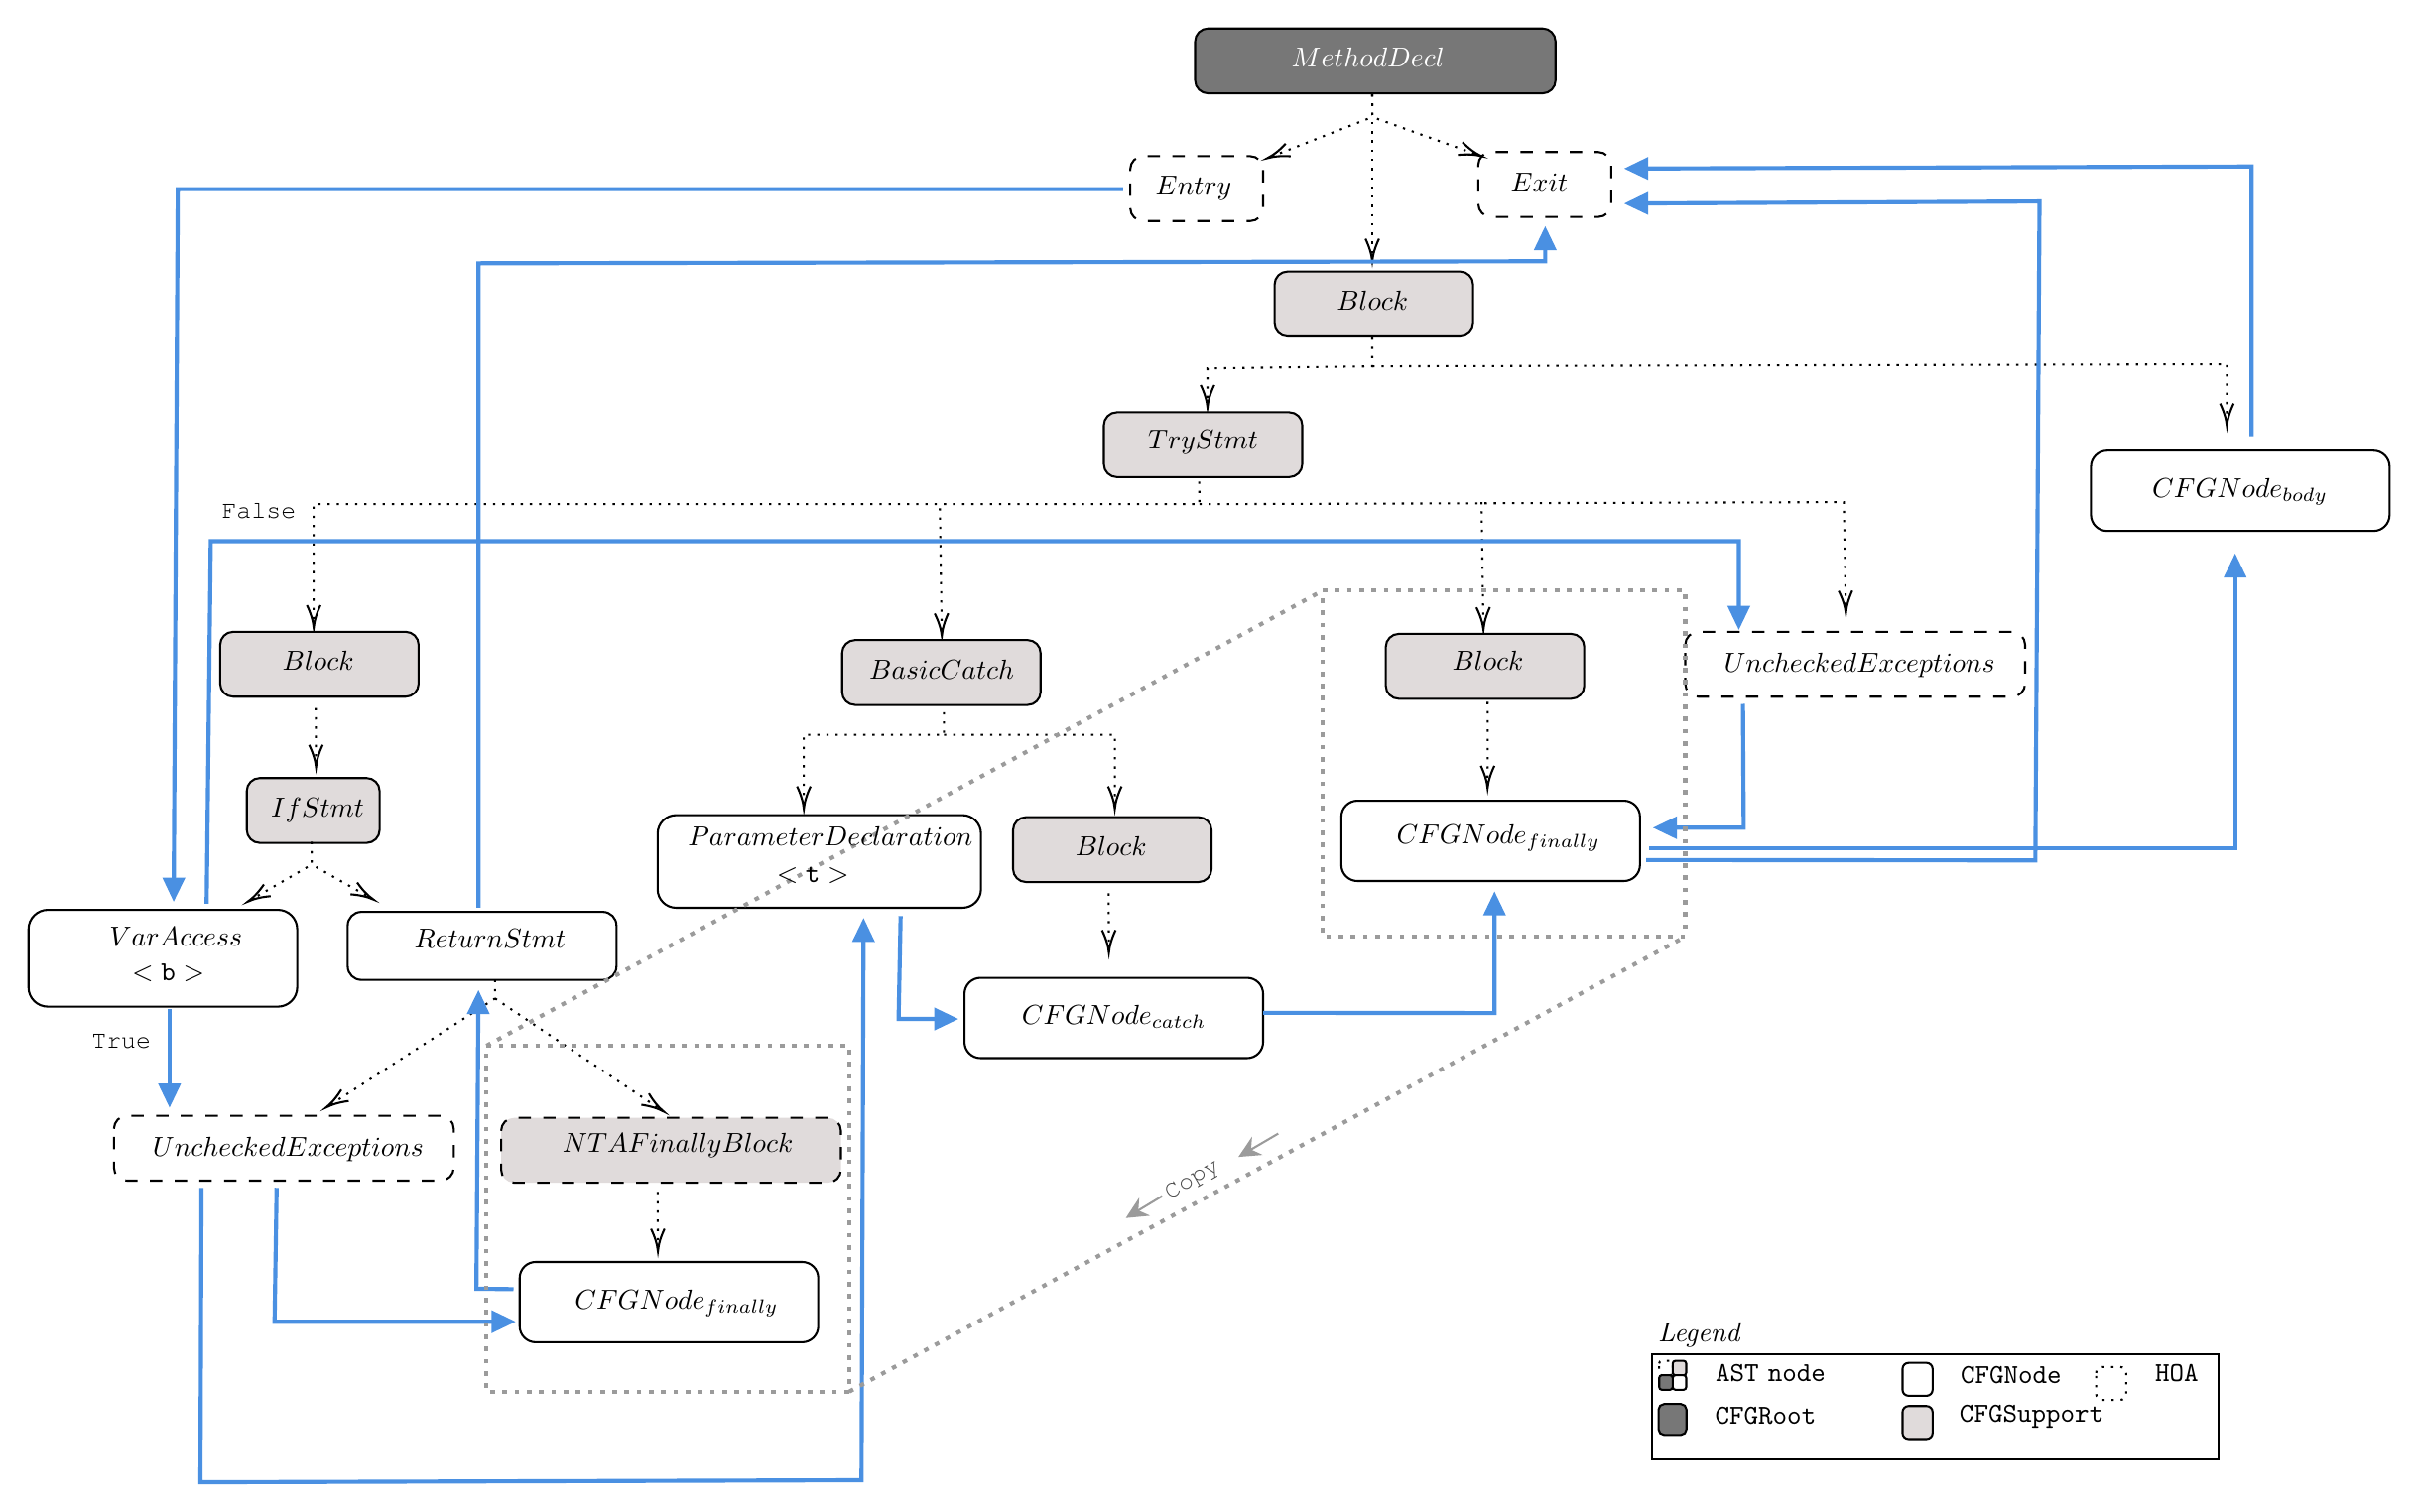
\begin{tikzpicture}[x=0.75pt,y=0.75pt,yscale=-1,xscale=1]
%uncomment if require: \path (0,954); %set diagram left start at 0, and has height of 954

%Rounded Rect [id:dp6052320426523271]
\draw  [fill={rgb, 255:red, 119; green, 119; blue, 119 }  ,fill opacity=1 ] (576,79.3) .. controls (576,75.82) and (578.82,73) .. (582.3,73) -- (744.7,73) .. controls (748.18,73) and (751,75.82) .. (751,79.3) -- (751,98.2) .. controls (751,101.68) and (748.18,104.5) .. (744.7,104.5) -- (582.3,104.5) .. controls (578.82,104.5) and (576,101.68) .. (576,98.2) -- cycle ;
%Rounded Rect [id:dp7366436282781997]
\draw  [dash pattern={on 4.5pt off 4.5pt}] (544.5,141.3) .. controls (544.5,137.82) and (547.32,135) .. (550.8,135) -- (602.7,135) .. controls (606.18,135) and (609,137.82) .. (609,141.3) -- (609,160.2) .. controls (609,163.68) and (606.18,166.5) .. (602.7,166.5) -- (550.8,166.5) .. controls (547.32,166.5) and (544.5,163.68) .. (544.5,160.2) -- cycle ;
%Rounded Rect [id:dp2901991809078346]
\draw  [dash pattern={on 4.5pt off 4.5pt}] (713.5,139.3) .. controls (713.5,135.82) and (716.32,133) .. (719.8,133) -- (771.7,133) .. controls (775.18,133) and (778,135.82) .. (778,139.3) -- (778,158.2) .. controls (778,161.68) and (775.18,164.5) .. (771.7,164.5) -- (719.8,164.5) .. controls (716.32,164.5) and (713.5,161.68) .. (713.5,158.2) -- cycle ;
%Straight Lines [id:da9218702965839638]
\draw  [dash pattern={on 0.84pt off 2.51pt}]  (662,105) -- (662.05,116.01) -- (612.86,135.27) ;
\draw [shift={(611,136)}, rotate = 338.62] [color={rgb, 255:red, 0; green, 0; blue, 0 }  ][line width=0.75]    (10.93,-3.29) .. controls (6.95,-1.4) and (3.31,-0.3) .. (0,0) .. controls (3.31,0.3) and (6.95,1.4) .. (10.93,3.29)   ;
%Straight Lines [id:da8010395012205194]
\draw  [dash pattern={on 0.84pt off 2.51pt}]  (662,105) -- (662.05,116.01) -- (713.12,134.32) ;
\draw [shift={(715,135)}, rotate = 199.73] [color={rgb, 255:red, 0; green, 0; blue, 0 }  ][line width=0.75]    (10.93,-3.29) .. controls (6.95,-1.4) and (3.31,-0.3) .. (0,0) .. controls (3.31,0.3) and (6.95,1.4) .. (10.93,3.29)   ;
%Rounded Rect [id:dp0365668300259846]
\draw  [fill={rgb, 255:red, 224; green, 219; blue, 219 }  ,fill opacity=1 ] (614.58,197.3) .. controls (614.58,193.82) and (617.4,191) .. (620.88,191) -- (704.65,191) .. controls (708.12,191) and (710.95,193.82) .. (710.95,197.3) -- (710.95,216.2) .. controls (710.95,219.68) and (708.12,222.5) .. (704.65,222.5) -- (620.88,222.5) .. controls (617.4,222.5) and (614.58,219.68) .. (614.58,216.2) -- cycle ;
%Straight Lines [id:da019749701866621838]
\draw  [dash pattern={on 0.84pt off 2.51pt}]  (662,223) -- (662,237) -- (582,238) -- (582,255) ;
\draw [shift={(582,257)}, rotate = 270] [color={rgb, 255:red, 0; green, 0; blue, 0 }  ][line width=0.75]    (10.93,-3.29) .. controls (6.95,-1.4) and (3.31,-0.3) .. (0,0) .. controls (3.31,0.3) and (6.95,1.4) .. (10.93,3.29)   ;
%Rounded Rect [id:dp1633328123499802]
\draw  [fill={rgb, 255:red, 224; green, 219; blue, 219 }  ,fill opacity=1 ] (531.67,265.63) .. controls (531.67,262.15) and (534.49,259.33) .. (537.97,259.33) -- (621.73,259.33) .. controls (625.21,259.33) and (628.03,262.15) .. (628.03,265.63) -- (628.03,284.53) .. controls (628.03,288.01) and (625.21,290.83) .. (621.73,290.83) -- (537.97,290.83) .. controls (534.49,290.83) and (531.67,288.01) .. (531.67,284.53) -- cycle ;
%Rounded Rect [id:dp24867915755586134]
\draw  [fill={rgb, 255:red, 224; green, 219; blue, 219 }  ,fill opacity=1 ] (115.5,443.3) .. controls (115.5,439.82) and (118.32,437) .. (121.8,437) -- (173.7,437) .. controls (177.18,437) and (180,439.82) .. (180,443.3) -- (180,462.2) .. controls (180,465.68) and (177.18,468.5) .. (173.7,468.5) -- (121.8,468.5) .. controls (118.32,468.5) and (115.5,465.68) .. (115.5,462.2) -- cycle ;
%Rounded Rect [id:dp0746395988364279]
\draw   (9.5,510.4) .. controls (9.5,505.21) and (13.71,501) .. (18.9,501) -- (130.6,501) .. controls (135.79,501) and (140,505.21) .. (140,510.4) -- (140,538.6) .. controls (140,543.79) and (135.79,548) .. (130.6,548) -- (18.9,548) .. controls (13.71,548) and (9.5,543.79) .. (9.5,538.6) -- cycle ;
%Straight Lines [id:da8214404714852102]
\draw  [dash pattern={on 0.84pt off 2.51pt}]  (578,293) -- (578.05,304.01) -- (148,304) -- (148,362) ;
\draw [shift={(148,364)}, rotate = 270] [color={rgb, 255:red, 0; green, 0; blue, 0 }  ][line width=0.75]    (10.93,-3.29) .. controls (6.95,-1.4) and (3.31,-0.3) .. (0,0) .. controls (3.31,0.3) and (6.95,1.4) .. (10.93,3.29)   ;
%Straight Lines [id:da9516705956971532]
\draw  [dash pattern={on 0.84pt off 2.51pt}]  (147,468) -- (147.05,479.01) -- (117.73,496) ;
\draw [shift={(116,497)}, rotate = 329.91999999999996] [color={rgb, 255:red, 0; green, 0; blue, 0 }  ][line width=0.75]    (10.93,-3.29) .. controls (6.95,-1.4) and (3.31,-0.3) .. (0,0) .. controls (3.31,0.3) and (6.95,1.4) .. (10.93,3.29)   ;
%Straight Lines [id:da5698232044281665]
\draw  [dash pattern={on 0.84pt off 2.51pt}]  (147,468) -- (147.05,479.01) -- (175.26,495.01) ;
\draw [shift={(177,496)}, rotate = 209.56] [color={rgb, 255:red, 0; green, 0; blue, 0 }  ][line width=0.75]    (10.93,-3.29) .. controls (6.95,-1.4) and (3.31,-0.3) .. (0,0) .. controls (3.31,0.3) and (6.95,1.4) .. (10.93,3.29)   ;
%Straight Lines [id:da6591561340961893]
\draw  [dash pattern={on 0.84pt off 2.51pt}]  (662,105) -- (662,184) ;
\draw [shift={(662,186)}, rotate = 270] [color={rgb, 255:red, 0; green, 0; blue, 0 }  ][line width=0.75]    (10.93,-3.29) .. controls (6.95,-1.4) and (3.31,-0.3) .. (0,0) .. controls (3.31,0.3) and (6.95,1.4) .. (10.93,3.29)   ;
%Rounded Rect [id:dp3889179480463789]
\draw  [dash pattern={on 4.5pt off 4.5pt}] (814,372.3) .. controls (814,368.82) and (816.82,366) .. (820.3,366) -- (972.7,366) .. controls (976.18,366) and (979,368.82) .. (979,372.3) -- (979,391.2) .. controls (979,394.68) and (976.18,397.5) .. (972.7,397.5) -- (820.3,397.5) .. controls (816.82,397.5) and (814,394.68) .. (814,391.2) -- cycle ;
%Rounded Rect [id:dp7590166547369378]
\draw  [fill={rgb, 255:red, 255; green, 255; blue, 255 }  ,fill opacity=1 ] (464,541.8) .. controls (464,537.49) and (467.49,534) .. (471.8,534) -- (601.2,534) .. controls (605.51,534) and (609,537.49) .. (609,541.8) -- (609,565.2) .. controls (609,569.51) and (605.51,573) .. (601.2,573) -- (471.8,573) .. controls (467.49,573) and (464,569.51) .. (464,565.2) -- cycle ;
%Rounded Rect [id:dp13372545457333695]
\draw   (164.5,508.6) .. controls (164.5,504.95) and (167.45,502) .. (171.1,502) -- (288.4,502) .. controls (292.05,502) and (295,504.95) .. (295,508.6) -- (295,528.4) .. controls (295,532.05) and (292.05,535) .. (288.4,535) -- (171.1,535) .. controls (167.45,535) and (164.5,532.05) .. (164.5,528.4) -- cycle ;
%Straight Lines [id:da10120384742733757]
\draw  [dash pattern={on 0.84pt off 2.51pt}]  (452.05,306.01) -- (452.97,366) ;
\draw [shift={(453,368)}, rotate = 269.12] [color={rgb, 255:red, 0; green, 0; blue, 0 }  ][line width=0.75]    (10.93,-3.29) .. controls (6.95,-1.4) and (3.31,-0.3) .. (0,0) .. controls (3.31,0.3) and (6.95,1.4) .. (10.93,3.29)   ;
%Straight Lines [id:da6751022167283701]
\draw  [dash pattern={on 0.84pt off 2.51pt}]  (578.05,304.01) -- (891,303) -- (891.96,355) ;
\draw [shift={(892,357)}, rotate = 268.94] [color={rgb, 255:red, 0; green, 0; blue, 0 }  ][line width=0.75]    (10.93,-3.29) .. controls (6.95,-1.4) and (3.31,-0.3) .. (0,0) .. controls (3.31,0.3) and (6.95,1.4) .. (10.93,3.29)   ;
%Rounded Rect [id:dp1694508010771657]
\draw  [fill={rgb, 255:red, 224; green, 219; blue, 219 }  ,fill opacity=1 ] (404.58,376.3) .. controls (404.58,372.82) and (407.4,370) .. (410.88,370) -- (494.65,370) .. controls (498.12,370) and (500.95,372.82) .. (500.95,376.3) -- (500.95,395.2) .. controls (500.95,398.68) and (498.12,401.5) .. (494.65,401.5) -- (410.88,401.5) .. controls (407.4,401.5) and (404.58,398.68) .. (404.58,395.2) -- cycle ;
%Rounded Rect [id:dp6643971026334665]
\draw  [fill={rgb, 255:red, 224; green, 219; blue, 219 }  ,fill opacity=1 ] (102.58,372.3) .. controls (102.58,368.82) and (105.4,366) .. (108.88,366) -- (192.65,366) .. controls (196.12,366) and (198.95,368.82) .. (198.95,372.3) -- (198.95,391.2) .. controls (198.95,394.68) and (196.12,397.5) .. (192.65,397.5) -- (108.88,397.5) .. controls (105.4,397.5) and (102.58,394.68) .. (102.58,391.2) -- cycle ;
%Straight Lines [id:da5017508889196973]
\draw  [dash pattern={on 0.84pt off 2.51pt}]  (149,403) -- (149.05,414.01) -- (149.13,429.81) ;
\draw [shift={(149.13,431.81)}, rotate = 269.73] [color={rgb, 255:red, 0; green, 0; blue, 0 }  ][line width=0.75]    (10.93,-3.29) .. controls (6.95,-1.4) and (3.31,-0.3) .. (0,0) .. controls (3.31,0.3) and (6.95,1.4) .. (10.93,3.29)   ;
%Rounded Rect [id:dp34186676051451803]
\draw  [fill={rgb, 255:red, 224; green, 219; blue, 219 }  ,fill opacity=1 ] (487.58,462.3) .. controls (487.58,458.82) and (490.4,456) .. (493.88,456) -- (577.65,456) .. controls (581.12,456) and (583.95,458.82) .. (583.95,462.3) -- (583.95,481.2) .. controls (583.95,484.68) and (581.12,487.5) .. (577.65,487.5) -- (493.88,487.5) .. controls (490.4,487.5) and (487.58,484.68) .. (487.58,481.2) -- cycle ;
%Straight Lines [id:da00038176688179125673]
\draw  [dash pattern={on 0.84pt off 2.51pt}]  (534,493) -- (534.05,504.01) -- (534.13,519.81) ;
\draw [shift={(534.13,521.81)}, rotate = 269.73] [color={rgb, 255:red, 0; green, 0; blue, 0 }  ][line width=0.75]    (10.93,-3.29) .. controls (6.95,-1.4) and (3.31,-0.3) .. (0,0) .. controls (3.31,0.3) and (6.95,1.4) .. (10.93,3.29)   ;
%Rounded Rect [id:dp4209817195306774]
\draw   (315,464) .. controls (315,459.03) and (319.03,455) .. (324,455) -- (463,455) .. controls (467.97,455) and (472,459.03) .. (472,464) -- (472,491) .. controls (472,495.97) and (467.97,500) .. (463,500) -- (324,500) .. controls (319.03,500) and (315,495.97) .. (315,491) -- cycle ;
%Straight Lines [id:da2379948200069697]
\draw  [dash pattern={on 0.84pt off 2.51pt}]  (454,405) -- (454.05,416.01) -- (386,416) -- (386,450) ;
\draw [shift={(386,452)}, rotate = 270] [color={rgb, 255:red, 0; green, 0; blue, 0 }  ][line width=0.75]    (10.93,-3.29) .. controls (6.95,-1.4) and (3.31,-0.3) .. (0,0) .. controls (3.31,0.3) and (6.95,1.4) .. (10.93,3.29)   ;
%Straight Lines [id:da9004148471132143]
\draw  [dash pattern={on 0.84pt off 2.51pt}]  (454.05,416.01) -- (537,416) -- (537,450) ;
\draw [shift={(537,452)}, rotate = 270] [color={rgb, 255:red, 0; green, 0; blue, 0 }  ][line width=0.75]    (10.93,-3.29) .. controls (6.95,-1.4) and (3.31,-0.3) .. (0,0) .. controls (3.31,0.3) and (6.95,1.4) .. (10.93,3.29)   ;
%Straight Lines [id:da7737763540695953]
\draw  [dash pattern={on 0.84pt off 2.51pt}]  (715.05,303.01) -- (715.97,363) ;
\draw [shift={(716,365)}, rotate = 269.12] [color={rgb, 255:red, 0; green, 0; blue, 0 }  ][line width=0.75]    (10.93,-3.29) .. controls (6.95,-1.4) and (3.31,-0.3) .. (0,0) .. controls (3.31,0.3) and (6.95,1.4) .. (10.93,3.29)   ;
%Rounded Rect [id:dp7437540797435133]
\draw  [fill={rgb, 255:red, 224; green, 219; blue, 219 }  ,fill opacity=1 ] (668.58,373.3) .. controls (668.58,369.82) and (671.4,367) .. (674.88,367) -- (758.65,367) .. controls (762.12,367) and (764.95,369.82) .. (764.95,373.3) -- (764.95,392.2) .. controls (764.95,395.68) and (762.12,398.5) .. (758.65,398.5) -- (674.88,398.5) .. controls (671.4,398.5) and (668.58,395.68) .. (668.58,392.2) -- cycle ;
%Straight Lines [id:da4653345052522305]
\draw  [dash pattern={on 0.84pt off 2.51pt}]  (718,400) -- (718.05,411.01) -- (718,440) ;
\draw [shift={(718,442)}, rotate = 270.1] [color={rgb, 255:red, 0; green, 0; blue, 0 }  ][line width=0.75]    (10.93,-3.29) .. controls (6.95,-1.4) and (3.31,-0.3) .. (0,0) .. controls (3.31,0.3) and (6.95,1.4) .. (10.93,3.29)   ;
%Straight Lines [id:da20327595857326908]
\draw  [dash pattern={on 0.84pt off 2.51pt}]  (662,237) -- (1077,236) -- (1077,264) ;
\draw [shift={(1077,266)}, rotate = 270] [color={rgb, 255:red, 0; green, 0; blue, 0 }  ][line width=0.75]    (10.93,-3.29) .. controls (6.95,-1.4) and (3.31,-0.3) .. (0,0) .. controls (3.31,0.3) and (6.95,1.4) .. (10.93,3.29)   ;
%Rounded Rect [id:dp6628949813345104]
\draw  [dash pattern={on 4.5pt off 4.5pt}] (51,607.3) .. controls (51,603.82) and (53.82,601) .. (57.3,601) -- (209.7,601) .. controls (213.18,601) and (216,603.82) .. (216,607.3) -- (216,626.2) .. controls (216,629.68) and (213.18,632.5) .. (209.7,632.5) -- (57.3,632.5) .. controls (53.82,632.5) and (51,629.68) .. (51,626.2) -- cycle ;
%Straight Lines [id:da09209016843774265]
\draw  [dash pattern={on 0.84pt off 2.51pt}]  (236,535) -- (236.05,544.01) -- (155.68,595.92) ;
\draw [shift={(154,597)}, rotate = 327.15] [color={rgb, 255:red, 0; green, 0; blue, 0 }  ][line width=0.75]    (10.93,-3.29) .. controls (6.95,-1.4) and (3.31,-0.3) .. (0,0) .. controls (3.31,0.3) and (6.95,1.4) .. (10.93,3.29)   ;
%Straight Lines [id:da6007896907634842]
\draw  [dash pattern={on 0.84pt off 2.51pt}]  (236.05,544.01) -- (316.34,597.89) ;
\draw [shift={(318,599)}, rotate = 213.86] [color={rgb, 255:red, 0; green, 0; blue, 0 }  ][line width=0.75]    (10.93,-3.29) .. controls (6.95,-1.4) and (3.31,-0.3) .. (0,0) .. controls (3.31,0.3) and (6.95,1.4) .. (10.93,3.29)   ;
%Straight Lines [id:da029673317319294124]
\draw  [dash pattern={on 0.84pt off 2.51pt}]  (315,638) -- (315.13,664.81) ;
\draw [shift={(315.13,666.81)}, rotate = 269.73] [color={rgb, 255:red, 0; green, 0; blue, 0 }  ][line width=0.75]    (10.93,-3.29) .. controls (6.95,-1.4) and (3.31,-0.3) .. (0,0) .. controls (3.31,0.3) and (6.95,1.4) .. (10.93,3.29)   ;
%Rounded Rect [id:dp08563744558423747]
\draw  [fill={rgb, 255:red, 224; green, 219; blue, 219 }  ,fill opacity=1 ][dash pattern={on 4.5pt off 4.5pt}] (239,608.3) .. controls (239,604.82) and (241.82,602) .. (245.3,602) -- (397.7,602) .. controls (401.18,602) and (404,604.82) .. (404,608.3) -- (404,627.2) .. controls (404,630.68) and (401.18,633.5) .. (397.7,633.5) -- (245.3,633.5) .. controls (241.82,633.5) and (239,630.68) .. (239,627.2) -- cycle ;
%Straight Lines [id:da10337967042371254]
\draw [color={rgb, 255:red, 74; green, 144; blue, 226 }  ,draw opacity=1 ][line width=1.5]    (541,151) -- (82,151) -- (80.02,493) ;
\draw [shift={(80,497)}, rotate = 270.33] [fill={rgb, 255:red, 74; green, 144; blue, 226 }  ,fill opacity=1 ][line width=0.08]  [draw opacity=0] (11.61,-5.58) -- (0,0) -- (11.61,5.58) -- cycle    ;
%Straight Lines [id:da038661732986791764]
\draw [color={rgb, 255:red, 74; green, 144; blue, 226 }  ,draw opacity=1 ][line width=1.5]    (840,361) -- (840,322) -- (98,322) -- (96,498) ;
\draw [shift={(840,365)}, rotate = 270] [fill={rgb, 255:red, 74; green, 144; blue, 226 }  ,fill opacity=1 ][line width=0.08]  [draw opacity=0] (11.61,-5.58) -- (0,0) -- (11.61,5.58) -- cycle    ;
%Straight Lines [id:da5286459154239997]
\draw [color={rgb, 255:red, 74; green, 144; blue, 226 }  ,draw opacity=1 ][line width=1.5]    (78,593) -- (78,549) ;
\draw [shift={(78,597)}, rotate = 270] [fill={rgb, 255:red, 74; green, 144; blue, 226 }  ,fill opacity=1 ][line width=0.08]  [draw opacity=0] (11.61,-5.58) -- (0,0) -- (11.61,5.58) -- cycle    ;
%Straight Lines [id:da36307512598343517]
\draw [color={rgb, 255:red, 74; green, 144; blue, 226 }  ,draw opacity=1 ][line width=1.5]    (242,701) -- (198,701) -- (129,701) -- (130,636) ;
\draw [shift={(246,701)}, rotate = 180] [fill={rgb, 255:red, 74; green, 144; blue, 226 }  ,fill opacity=1 ][line width=0.08]  [draw opacity=0] (11.61,-5.58) -- (0,0) -- (11.61,5.58) -- cycle    ;
%Straight Lines [id:da438540135636014]
\draw [color={rgb, 255:red, 74; green, 144; blue, 226 }  ,draw opacity=1 ][line width=1.5]    (227.97,544) -- (227,685) -- (245,685.2) ;
\draw [shift={(228,540)}, rotate = 90.4] [fill={rgb, 255:red, 74; green, 144; blue, 226 }  ,fill opacity=1 ][line width=0.08]  [draw opacity=0] (11.61,-5.58) -- (0,0) -- (11.61,5.58) -- cycle    ;
%Straight Lines [id:da04549690537686513]
\draw [color={rgb, 255:red, 74; green, 144; blue, 226 }  ,draw opacity=1 ][line width=1.5]    (746,173) -- (746,186) -- (228,187) -- (228,500) ;
\draw [shift={(746,169)}, rotate = 90] [fill={rgb, 255:red, 74; green, 144; blue, 226 }  ,fill opacity=1 ][line width=0.08]  [draw opacity=0] (11.61,-5.58) -- (0,0) -- (11.61,5.58) -- cycle    ;
%Straight Lines [id:da47146018862646266]
\draw [color={rgb, 255:red, 74; green, 144; blue, 226 }  ,draw opacity=1 ][line width=1.5]    (414.99,509) -- (414,778) -- (93,779) -- (93.5,636) ;
\draw [shift={(415,505)}, rotate = 90.21] [fill={rgb, 255:red, 74; green, 144; blue, 226 }  ,fill opacity=1 ][line width=0.08]  [draw opacity=0] (11.61,-5.58) -- (0,0) -- (11.61,5.58) -- cycle    ;
%Straight Lines [id:da09435969977156955]
\draw [color={rgb, 255:red, 74; green, 144; blue, 226 }  ,draw opacity=1 ][line width=1.5]    (457,554) -- (432,554) -- (433,504) ;
\draw [shift={(461,554)}, rotate = 180] [fill={rgb, 255:red, 74; green, 144; blue, 226 }  ,fill opacity=1 ][line width=0.08]  [draw opacity=0] (11.61,-5.58) -- (0,0) -- (11.61,5.58) -- cycle    ;
%Straight Lines [id:da40869470254178497]
\draw [color={rgb, 255:red, 74; green, 144; blue, 226 }  ,draw opacity=1 ][line width=1.5]    (721.37,496.13) -- (721.37,551.13) -- (609,551) ;
\draw [shift={(721.37,492.13)}, rotate = 90] [fill={rgb, 255:red, 74; green, 144; blue, 226 }  ,fill opacity=1 ][line width=0.08]  [draw opacity=0] (11.61,-5.58) -- (0,0) -- (11.61,5.58) -- cycle    ;
%Straight Lines [id:da9149453592330149]
\draw [color={rgb, 255:red, 74; green, 144; blue, 226 }  ,draw opacity=1 ][line width=1.5]    (802.37,461.13) -- (842.37,461.13) -- (842,401) ;
\draw [shift={(798.37,461.13)}, rotate = 0] [fill={rgb, 255:red, 74; green, 144; blue, 226 }  ,fill opacity=1 ][line width=0.08]  [draw opacity=0] (11.61,-5.58) -- (0,0) -- (11.61,5.58) -- cycle    ;
%Straight Lines [id:da9771253399321245]
\draw [color={rgb, 255:red, 74; green, 144; blue, 226 }  ,draw opacity=1 ][line width=1.5]    (1081,332) -- (1081,471) -- (796.37,471) ;
\draw [shift={(1081,328)}, rotate = 90] [fill={rgb, 255:red, 74; green, 144; blue, 226 }  ,fill opacity=1 ][line width=0.08]  [draw opacity=0] (11.61,-5.58) -- (0,0) -- (11.61,5.58) -- cycle    ;
%Straight Lines [id:da39472224978063597]
\draw [color={rgb, 255:red, 74; green, 144; blue, 226 }  ,draw opacity=1 ][line width=1.5]    (788.37,157.98) -- (986,157) -- (984,477) -- (795,476.8) ;
\draw [shift={(784.37,158)}, rotate = 359.72] [fill={rgb, 255:red, 74; green, 144; blue, 226 }  ,fill opacity=1 ][line width=0.08]  [draw opacity=0] (11.61,-5.58) -- (0,0) -- (11.61,5.58) -- cycle    ;
%Straight Lines [id:da9377433477264157]
\draw [color={rgb, 255:red, 74; green, 144; blue, 226 }  ,draw opacity=1 ][line width=1.5]    (788.37,140.99) -- (1089,140) -- (1089,271) ;
\draw [shift={(784.37,141)}, rotate = 359.81] [fill={rgb, 255:red, 74; green, 144; blue, 226 }  ,fill opacity=1 ][line width=0.08]  [draw opacity=0] (11.61,-5.58) -- (0,0) -- (11.61,5.58) -- cycle    ;
%Rounded Rect [id:dp9976397465711901]
\draw  [fill={rgb, 255:red, 255; green, 255; blue, 255 }  ,fill opacity=1 ] (248,679.8) .. controls (248,675.49) and (251.49,672) .. (255.8,672) -- (385.2,672) .. controls (389.51,672) and (393,675.49) .. (393,679.8) -- (393,703.2) .. controls (393,707.51) and (389.51,711) .. (385.2,711) -- (255.8,711) .. controls (251.49,711) and (248,707.51) .. (248,703.2) -- cycle ;
%Rounded Rect [id:dp8082455595328036]
\draw  [fill={rgb, 255:red, 255; green, 255; blue, 255 }  ,fill opacity=1 ] (647,455.8) .. controls (647,451.49) and (650.49,448) .. (654.8,448) -- (784.2,448) .. controls (788.51,448) and (792,451.49) .. (792,455.8) -- (792,479.2) .. controls (792,483.51) and (788.51,487) .. (784.2,487) -- (654.8,487) .. controls (650.49,487) and (647,483.51) .. (647,479.2) -- cycle ;
%Rounded Rect [id:dp665384939346158]
\draw  [fill={rgb, 255:red, 255; green, 255; blue, 255 }  ,fill opacity=1 ] (1011,285.8) .. controls (1011,281.49) and (1014.49,278) .. (1018.8,278) -- (1148.2,278) .. controls (1152.51,278) and (1156,281.49) .. (1156,285.8) -- (1156,309.2) .. controls (1156,313.51) and (1152.51,317) .. (1148.2,317) -- (1018.8,317) .. controls (1014.49,317) and (1011,313.51) .. (1011,309.2) -- cycle ;
%Shape: Rectangle [id:dp7829149877739602]
\draw  [color={rgb, 255:red, 155; green, 155; blue, 155 }  ,draw opacity=1 ][dash pattern={on 1.69pt off 2.76pt}][line width=1.5]  (637.88,346) -- (814,346) -- (814,514) -- (637.88,514) -- cycle ;
%Shape: Rectangle [id:dp10471447597627126]
\draw  [color={rgb, 255:red, 155; green, 155; blue, 155 }  ,draw opacity=1 ][dash pattern={on 1.69pt off 2.76pt}][line width=1.5]  (231.88,567) -- (408,567) -- (408,735) -- (231.88,735) -- cycle ;
%Straight Lines [id:da35435821453029226]
\draw [color={rgb, 255:red, 155; green, 155; blue, 155 }  ,draw opacity=1 ][line width=1.5]  [dash pattern={on 1.69pt off 2.76pt}]  (408,735) -- (814,514) ;
%Straight Lines [id:da5252422896309856]
\draw [color={rgb, 255:red, 155; green, 155; blue, 155 }  ,draw opacity=1 ][line width=1.5]  [dash pattern={on 1.69pt off 2.76pt}]  (231.88,567) -- (637.88,346) ;
%Straight Lines [id:da904564732091522]
\draw [color={rgb, 255:red, 155; green, 155; blue, 155 }  ,draw opacity=1 ]   (560,640) -- (544.9,649.12) ;
\draw [shift={(542.33,650.67)}, rotate = 328.88] [fill={rgb, 255:red, 155; green, 155; blue, 155 }  ,fill opacity=1 ][line width=0.08]  [draw opacity=0] (10.72,-5.15) -- (0,0) -- (10.72,5.15) -- (7.12,0) -- cycle    ;
%Straight Lines [id:da8633137161207692]
\draw [color={rgb, 255:red, 155; green, 155; blue, 155 }  ,draw opacity=1 ]   (616.33,609.67) -- (599.59,619.48) ;
\draw [shift={(597,621)}, rotate = 329.62] [fill={rgb, 255:red, 155; green, 155; blue, 155 }  ,fill opacity=1 ][line width=0.08]  [draw opacity=0] (10.72,-5.15) -- (0,0) -- (10.72,5.15) -- (7.12,0) -- cycle    ;
%Shape: Rectangle [id:dp7726792143244623]
\draw   (798,717) -- (1073,717) -- (1073,768) -- (798,768) -- cycle ;
%Rounded Rect [id:dp45744152384191206]
\draw  [fill={rgb, 255:red, 255; green, 255; blue, 255 }  ,fill opacity=1 ] (919.49,723.92) .. controls (919.49,722.31) and (920.8,721) .. (922.41,721) -- (931.19,721) .. controls (932.8,721) and (934.11,722.31) .. (934.11,723.92) -- (934.11,734.08) .. controls (934.11,735.69) and (932.8,737) .. (931.19,737) -- (922.41,737) .. controls (920.8,737) and (919.49,735.69) .. (919.49,734.08) -- cycle ;
%Rounded Rect [id:dp46264916204068907]
\draw  [fill={rgb, 255:red, 119; green, 119; blue, 119 }  ,fill opacity=1 ] (801.01,743.72) .. controls (801.01,742.22) and (802.22,741) .. (803.72,741) -- (811.87,741) .. controls (813.37,741) and (814.59,742.22) .. (814.59,743.72) -- (814.59,753.28) .. controls (814.59,754.78) and (813.37,756) .. (811.87,756) -- (803.72,756) .. controls (802.22,756) and (801.01,754.78) .. (801.01,753.28) -- cycle ;
%Rounded Rect [id:dp18098601440359496]
\draw  [fill={rgb, 255:red, 224; green, 219; blue, 219 }  ,fill opacity=1 ] (919.49,744.92) .. controls (919.49,743.31) and (920.8,742) .. (922.41,742) -- (931.19,742) .. controls (932.8,742) and (934.11,743.31) .. (934.11,744.92) -- (934.11,755.08) .. controls (934.11,756.69) and (932.8,758) .. (931.19,758) -- (922.41,758) .. controls (920.8,758) and (919.49,756.69) .. (919.49,755.08) -- cycle ;
%Rounded Rect [id:dp24736728041755873]
\draw  [fill={rgb, 255:red, 255; green, 255; blue, 255 }  ,fill opacity=1 ][dash pattern={on 0.84pt off 2.51pt}] (801.3,721.31) .. controls (801.3,720.59) and (801.89,720) .. (802.61,720) -- (806.55,720) .. controls (807.28,720) and (807.87,720.59) .. (807.87,721.31) -- (807.87,725.77) .. controls (807.87,726.49) and (807.28,727.08) .. (806.55,727.08) -- (802.61,727.08) .. controls (801.89,727.08) and (801.3,726.49) .. (801.3,725.77) -- cycle ;
%Rounded Rect [id:dp8619496982908982]
\draw  [fill={rgb, 255:red, 224; green, 219; blue, 219 }  ,fill opacity=1 ] (807.9,721.31) .. controls (807.9,720.59) and (808.49,720) .. (809.21,720) -- (813.16,720) .. controls (813.88,720) and (814.47,720.59) .. (814.47,721.31) -- (814.47,725.77) .. controls (814.47,726.49) and (813.88,727.08) .. (813.16,727.08) -- (809.21,727.08) .. controls (808.49,727.08) and (807.9,726.49) .. (807.9,725.77) -- cycle ;
%Rounded Rect [id:dp2369415791405316]
\draw  [fill={rgb, 255:red, 255; green, 255; blue, 255 }  ,fill opacity=1 ] (807.9,728.31) .. controls (807.9,727.59) and (808.49,727) .. (809.21,727) -- (813.16,727) .. controls (813.88,727) and (814.47,727.59) .. (814.47,728.31) -- (814.47,732.77) .. controls (814.47,733.49) and (813.88,734.08) .. (813.16,734.08) -- (809.21,734.08) .. controls (808.49,734.08) and (807.9,733.49) .. (807.9,732.77) -- cycle ;
%Rounded Rect [id:dp24376981804797926]
\draw  [fill={rgb, 255:red, 119; green, 119; blue, 119 }  ,fill opacity=1 ] (801.33,728.31) .. controls (801.33,727.59) and (801.92,727) .. (802.64,727) -- (806.58,727) .. controls (807.31,727) and (807.9,727.59) .. (807.9,728.31) -- (807.9,732.77) .. controls (807.9,733.49) and (807.31,734.08) .. (806.58,734.08) -- (802.64,734.08) .. controls (801.92,734.08) and (801.33,733.49) .. (801.33,732.77) -- cycle ;
%Rounded Rect [id:dp9982976151547778]
\draw  [fill={rgb, 255:red, 255; green, 255; blue, 255 }  ,fill opacity=1 ][dash pattern={on 0.84pt off 2.51pt}] (1013.49,725.92) .. controls (1013.49,724.31) and (1014.8,723) .. (1016.41,723) -- (1025.19,723) .. controls (1026.8,723) and (1028.11,724.31) .. (1028.11,725.92) -- (1028.11,736.08) .. controls (1028.11,737.69) and (1026.8,739) .. (1025.19,739) -- (1016.41,739) .. controls (1014.8,739) and (1013.49,737.69) .. (1013.49,736.08) -- cycle ;

% Text Node
\draw (621.33,81) node [anchor=north west][inner sep=0.75pt]  [color={rgb, 255:red, 255; green, 255; blue, 255 }  ,opacity=1 ]  {$MethodDecl$};
% Text Node
\draw (555.33,143) node [anchor=north west][inner sep=0.75pt]    {$Entry$};
% Text Node
\draw (727.8,141.75) node [anchor=north west][inner sep=0.75pt]    {$Exit$};
% Text Node
\draw (643.33,199) node [anchor=north west][inner sep=0.75pt]    {$Block$};
% Text Node
\draw (551.67,266.63) node [anchor=north west][inner sep=0.75pt]    {$TryStmt$};
% Text Node
\draw (125.8,445) node [anchor=north west][inner sep=0.75pt]    {$IfStmt$};
% Text Node
\draw (47.33,508) node [anchor=north west][inner sep=0.75pt]    {$VarAccess$};
% Text Node
\draw (58.3,526) node [anchor=north west][inner sep=0.75pt]    {$\mathtt{< b >}$};
% Text Node
\draw (831.3,375) node [anchor=north west][inner sep=0.75pt]    {$UncheckedExceptions$};
% Text Node
\draw (490.3,546) node [anchor=north west][inner sep=0.75pt]  [color={rgb, 255:red, 0; green, 0; blue, 0 }  ,opacity=1 ]  {$CFGNode_{catch}$};
% Text Node
\draw (195.33,509) node [anchor=north west][inner sep=0.75pt]    {$ReturnStmt$};
% Text Node
\draw (416.33,378) node [anchor=north west][inner sep=0.75pt]    {$BasicCatch$};
% Text Node
\draw (131.33,374) node [anchor=north west][inner sep=0.75pt]    {$Block$};
% Text Node
\draw (516.33,464) node [anchor=north west][inner sep=0.75pt]    {$Block$};
% Text Node
\draw (328.2,459) node [anchor=north west][inner sep=0.75pt]    {$ParameterDeclaration$};
% Text Node
\draw (371.3,479) node [anchor=north west][inner sep=0.75pt]    {$\mathtt{< t >}$};
% Text Node
\draw (699.33,374) node [anchor=north west][inner sep=0.75pt]    {$Block$};
% Text Node
\draw (68.3,610) node [anchor=north west][inner sep=0.75pt]    {$UncheckedExceptions$};
% Text Node
\draw (267.3,608) node [anchor=north west][inner sep=0.75pt]    {$NTAFinallyBlock$};
% Text Node
\draw (99,302) node [anchor=north west][inner sep=0.75pt]   [align=left] {\begin{minipage}[lt]{31.290625000000002pt}\setlength\topsep{0pt}
\begin{center}
{\fontfamily{pcr}\selectfont {\small False}}
\end{center}

\end{minipage}};
% Text Node
\draw (36,560) node [anchor=north west][inner sep=0.75pt]   [align=left] {\begin{minipage}[lt]{25.574375000000003pt}\setlength\topsep{0pt}
\begin{center}
{\fontfamily{pcr}\selectfont {\small True}}
\end{center}

\end{minipage}};
% Text Node
\draw (273.3,684) node [anchor=north west][inner sep=0.75pt]  [color={rgb, 255:red, 0; green, 0; blue, 0 }  ,opacity=1 ]  {$CFGNode_{finally}$};
% Text Node
\draw (672.3,458) node [anchor=north west][inner sep=0.75pt]  [color={rgb, 255:red, 0; green, 0; blue, 0 }  ,opacity=1 ]  {$CFGNode_{finally}$};
% Text Node
\draw (1039.3,290) node [anchor=north west][inner sep=0.75pt]  [color={rgb, 255:red, 0; green, 0; blue, 0 }  ,opacity=1 ]  {$CFGNode_{body}$};
% Text Node
\draw (552.46,638.32) node [anchor=north west][inner sep=0.75pt]  [color={rgb, 255:red, 74; green, 74; blue, 74 }  ,opacity=1 ,rotate=-329.71] [align=left] {\begin{minipage}[lt]{31.290625000000002pt}\setlength\topsep{0pt}
\begin{center}
{\fontfamily{pcr}\selectfont {\small Copy }}
\end{center}

\end{minipage}};
% Text Node
\draw (827,741.33) node [anchor=north west][inner sep=0.75pt]    {$\mathtt{CFGRoot}$};
% Text Node
\draw (946.23,721.33) node [anchor=north west][inner sep=0.75pt]    {$\mathtt{CFGNode}$};
% Text Node
\draw (945.72,740.33) node [anchor=north west][inner sep=0.75pt]    {$\mathtt{CFGSupport}$};
% Text Node
\draw (827.23,720.33) node [anchor=north west][inner sep=0.75pt]    {$\mathtt{AST\ node}$};
% Text Node
\draw (799.35,700) node [anchor=north west][inner sep=0.75pt]   [align=left] {\textit{Legend}};
% Text Node
\draw (1040.72,720.33) node [anchor=north west][inner sep=0.75pt]    {$\mathtt{HOA}$};


\end{tikzpicture}

%	        }
%	\end{subfigure}
%\caption{Example of use of NTAs \astnode{UncheckedExceptions} and \astnode{NTAFinallyBlock}.}\label{fig:unchecked-exn}
%\end{figure*}
%\subsection{Possible improvements}
%A further improvement, which is not implemented in \intraj, can be reifying
%the implicit boxing and unboxing operations of the primitive types with their
%respective wrappers, i.e., \code{Integer} and \code{int} or \code{Boolean} and
%\code{boolean}.
%\unsure{IR:If we decided to keep this subsection, then we can think of possible improvements.}
%Modelling these operations can help detect occurrences of \code{NullPointerExceptions}
%in case  a null wrapper is unboxed.
%\unsure{IR:maybe here we can discuss the 'refine' of  equations.}
%\CR{I couldn't find any references to Figure~\ref{fig:unchecked-exn}?}




